\chapter{留数定理}
留数是复变函数论中的重要概念之一.
留数定理是柯西积分理论的继续.
它们和计算复函数的围线积分问题有着密切的关系.
本章先叙述有关留数的一般理论,然后介绍留数理论在计算积分和考察函数零点分布状况中的应用.

\section{留数定理}
\subsection{留数的定义及计算方法}
我们知道,若有限点\(a\)是函数\(f(z)\)的解析点,围线\(\Gamma\)全在点\(a\)的某邻域内并包围点\(a\),则根据\hyperref[theorem:解析函数的积分表示.柯西积分定理]{柯西积分定理},有\[
\int_\Gamma f(z) \dd{z} = 0.
\]

若有限点\(a\)是\(f(z)\)的一个孤立奇点,则当围线\(\Gamma\)全在点\(a\)的某去心邻域\(U(a,R)\)内且包围点\(a\)时,积分\(\int_\Gamma f(z) \dd{z}\)的值通常不为零.
事实上,设在点\(a\)的某去心邻域\(\mathring{U}(a,R)\)内,\(f(z)\)的罗朗展式为\[
f(z) = \sum_{n=-\infty}^{+\infty} C_n (z-a)^n,
\]其中\(C_n\ (n=0,\pm1,\pm2,\dotsc)\)是复常数.
将上式等号两端沿\(\Gamma\)积分,
并利用\hyperref[theorem:解析函数的级数表示.一致收敛级数的基本性质2]{逐项积分定理}及
重要积分 \labelcref{equation:解析函数的积分表示.重要积分1} \[
	\int_\Gamma (z-a)^n \dd{z} = \left\{ \begin{array}{cl}
		2\pi\iu, & n=-1, \\
		0,& n\in\mathbb{Z}-\{-1\},
	\end{array} \right.
\]
可得\[
	\int_\Gamma f(z) \dd{z} = 2\pi\iu C_{-1}.
\]
也就是说,将\(f(z)\)的罗朗展式沿围线\(\Gamma\)积分后
将会只留下\((z-a)\)的负一次幂项积分不为零,
其余所有项积分通通为零.

由此可见,\(C_{-1}\)在罗朗展式的各个系数中具有独特的地位.
若不计因子\(2\pi\iu\),它实质上表现的是围线积分\(\int_\Gamma f(z) \dd{z}\)的值.

\begin{definition}
设有限点\(a\)为函数\(f(z)\)的一个孤立奇点,设\(f(z)\)在点\(a\)的去心邻域\(\mathring{U}(a,R)\)内解析,取围线\(\Gamma: \abs{z-a}=\rho\in(0,R)\),则称积分\[
\frac{1}{2\pi\iu} \int_\Gamma f(z) \dd{z}
\]为\(f(z)\)在点\(a\)的\DefineConcept{留数}(residue;又称作\DefineConcept{残数}),记作\(\Res_{z=a} f(z)\),即\begin{equation}\label{equation:留数定理.留数定义1}
\Res_{z=a} f(z)
= \frac{1}{2\pi\iu} \int_\Gamma f(z) \dd{z}
\quad(0<\rho<R).
\end{equation}
\end{definition}
根据\hyperref[theorem:解析函数的积分表示.多连通区域的柯西积分定理]{多连通区域上的柯西积分定理}以及前面的讨论可知,\begin{equation}\label{equation:留数定理.留数定义2}
\Res_{z=a} f(z) = C_{-1},
\end{equation}
其中\(C_{-1}\)为\(f(z)\)在点\(a\)去心邻域内罗朗展式的负一次幂系数.
显然,\cref{equation:留数定理.留数定义2} 也可作为\(f(z)\)在其孤立奇点\(a\)处的留数定义.

\begin{definition}
设\(z=\infty\)是函数\(f(z)\)的孤立奇点,
设\(f(z)\)在点\(\infty\)的去心邻域\(0 \leq r < \abs{z} < +\infty\)内解析.
取围线\(\Gamma: \abs{z} = \rho\in(r,+\infty)\),
则称积分\[
	\frac{1}{2\pi\iu} \int_{\Gamma^-} f(z) \dd{z}
\]为“\(f(z)\)在无穷远点\(\infty\)的留数”,
记为\(\Res_{z=\infty} f(z)\),
即\begin{equation}\label{equation:留数定理.留数定义3}
\Res_{z=\infty} f(z)
= \frac{1}{2\pi\iu} \int_{\Gamma^-} f(z) \dd{z}.
\end{equation}
\end{definition}
假设\(f(z)\)在孤立奇点\(\infty\)的去心邻域内可展成罗朗级数\[
f(z) = \sum_{n=-\infty}^\infty C_n z^n,
\]其中\(C_n\ (n=0,\pm1,\pm2,\dotsc)\)是复常数.
由\hyperref[theorem:解析函数的级数表示.一致收敛级数的基本性质2]{逐项积分定理}及重要积分 \labelcref{equation:解析函数的积分表示.重要积分1} 可知,\begin{equation}\label{equation:留数定理.留数定义4}
\Res_{z=\infty} f(z) = - C_{-1}.
\end{equation}
也就是说,\(\Res_{z=\infty} f(z)\)等于\(f(z)\)在点\(\infty\)的罗朗展式中\(\frac{1}{z}\)项系数的相反数.

这样,当我们知道点\(a\)是\(f(z)\)的孤立奇点时,不论点\(a\)是有限点还是\(\infty\),也不论点\(a\)是三类孤立奇点中的哪一种,我们总可以用罗朗展开的方法,按\cref{equation:留数定理.留数定义2} 或\cref{equation:留数定理.留数定义4} 求出\(f(z)\)在点\(a\)的留数.

\begin{property}
若\(a\)是可去奇点,且\(a\neq\infty\),则有\(\Res_{z=a} f(z) = 0\).
\end{property}

\begin{example}
函数\(f(z) = 1 + \frac{1}{z}\)在无穷远点\(\infty\)处解析,但\(\Res_{z=\infty} f(z) = -1\).
此例说明,无穷远点\(\infty\)作为任意复变函数\(f(z)\)的可去奇点时,\(f(z)\)的留数不一定是零.
\end{example}

\begin{property}
若\(a\neq\infty\)是\(f(z)\)的\(m\ (m\geq1)\)阶极点,则\(f(z)\)在点\(a\)的留数为\begin{equation}\label{equation:留数定理.函数在极点的留数1}
\Res_{z=a} f(z)
= \frac{1}{(m-1)!} \lim_{z \to a} \dv[m-1]{z} \{ (z-a)^m f(z) \}.
\end{equation}
特别地,当\(m=1\)时,\begin{equation}\label{equation:留数定理.函数在极点的留数2}
\Res_{z=a} f(z)
= \lim_{z \to a} [(z-a) f(z)].
\end{equation}
\begin{proof}
当有限点\(a\)为\(f(z)\)的\(m\)阶极点时,\(f(z)\)在点的去心邻域内可表成\begin{equation}\label{equation:留数定理.函数在极点的留数.辅助1式}
f(z) = \frac{1}{(z-a)^m} g(z),
\end{equation}
其中\(g(z)\)在点\(a\)是解析的,且\(g(a)\neq0\),\(g(z)\)在点\(a\)的邻域内可展成泰勒级数\[
g(z) = \sum_{n=0}^\infty \frac{1}{n!} g^{(n)}(a) (z-a)^n,
\]于是由\hyperref[equation:解析函数的积分表示.柯西高阶导数公式]{柯西高阶导数公式}\begin{equation}\label{equation:留数定理.函数在极点的留数.辅助2式}
\Res_{z=a} f(z) = C_{-1}
= \frac{1}{2\pi\iu} \int_{\abs{z-a}=\rho} \frac{g(z)}{(z-a)^m} \dd{z}
= \frac{1}{(m-1)!} g^{(m-1)}(a).
\end{equation}
由于\cref{equation:留数定理.函数在极点的留数.辅助1式} 中的\(g(z)\)在点\(a\)解析,
所以\[
g^{(m-1)}(a) = \lim_{z \to a} g^{(m-1)}(z)
= \lim_{z \to a} [(z-a)^m f(z)],
\]
因此\cref{equation:留数定理.函数在极点的留数.辅助2式}
即\cref{equation:留数定理.函数在极点的留数1}.

当\((z-a)^m f(z)\)中的\((z-a)^m\)因子能从\(f(z)\)中消去时,
就在消去后直接用\cref{equation:留数定理.函数在极点的留数.辅助2式}
计算\(\Res_{z=a} f(z)\),
否则才用极限等式 \labelcref{equation:留数定理.函数在极点的留数1} 计算.
这样做较为省事一些.

若\(f(z) = \frac{\phi(z)}{\psi(z)}\),
\(\phi(z)\)及\(\psi(z)\)在点\(a\)解析,且\(\phi(a)\neq0\),
\(\psi(a)=0\),\(\psi'(a)\neq0\),则\(a\)为\(f(z)\)的一阶极点,
于是\[
	\Res_{z=a} f(z)
	= \lim_{z \to a} (z-a) \frac{\phi(z)}{\psi(z)}
	= \lim_{z \to a} \frac{\phi(z)}{\frac{\psi(z)-\psi(a)}{z-a}}
	= \frac{\phi(a)}{\psi'(a)},
\]
即\begin{equation}\label{equation:留数定理.函数在极点的留数3}
	\Res_{z=a} f(z)
	= \frac{\phi(a)}{\psi'(a)}.
\end{equation}
这也是计算一阶极点留数的一个简便公式.
\end{proof}
\end{property}

\subsection{留数定理}
\begin{theorem}[柯西留数定理]\label{theorem:留数定理.柯西留数定理}
若\(f(z)\)在围线或复围线\(\Gamma\)所围区域\(D\)内除有限个奇点\(\AutoTuple{a}{n}\)外解析,在闭域\(\overline{D}=D+\Gamma\)上除\(\AutoTuple{a}{n}\)外连续,则\begin{equation}\label{equation:留数定理.柯西留数定理}
\int_\Gamma f(z) \dd{z}
= 2\pi\iu \sum_{k=1}^n \Res_{z=a_k} f(z).
\end{equation}
\begin{proof}
在\(D\)内以\(a_k\ (k=1,2,\dotsc,n)\)为中心作半径充分小的圆周\(\Gamma_k\),使得每个\(\Gamma_k\)都在其余小圆周的外部(即\(I(\Gamma_i) \cap I(\Gamma_j) = \emptyset\ (i \neq j)\)),而所有的小圆周又都在\(D\)的内部(即\(\bigcup_k I(\Gamma_k) \subseteq I(\Gamma)\)).
由\hyperref[theorem:解析函数的积分表示.多连通区域的柯西积分定理]{多连通区域上的柯西积分定理},有\[
\int_\Gamma f(z) \dd{z}
= \sum_{k=1}^n \int_{\Gamma_k} f(z) \dd{z}.
\]但按留数定义\[
\int_{\Gamma_k} f(z) \dd{z} = 2\pi\iu \Res_{z=a_k} f(z).
\]所以\cref{theorem:留数定理.柯西留数定理} 成立.
\end{proof}
\end{theorem}
柯西留数定理把计算围线积分的整体问题,化成了计算围线内部各孤立奇点处留数的局部问题.
这是留数定理的实质.
这里也表现了解析函数的特性.
利用这种特性,一方面可以用来计算围线积分;
另一方面,我们后面将看到,可以用来考查解析函数的零点分布状况.

\begin{theorem}\label{theorem:留数定理.孤立奇点的留数之和}
若\(f(z)\)在全平面\(\mathbb{C}\)上除有限个点\(\AutoTuple{a}{n}\)外解析,点\(\infty\)也为\(f(z)\)的孤立奇点,则\begin{equation}\label{equation:留数定理.孤立奇点的留数之和}
\sum_{k=1}^n \Res_{z=a_k} f(z) + \Res_{z=\infty} f(z) = 0.
\end{equation}也就是说,\(f(z)\)所有孤立奇点的留数之和为零.
\begin{proof}
以原点为心,作半径\(R\)充分大的圆周\(\Gamma\),使得\(\Gamma\)的内部包括\(\AutoTuple{a}{n}\).
由\cref{theorem:留数定理.柯西留数定理},\[
\int_\Gamma f(z) \dd{z}
= 2\pi\iu \sum_{k=1}^n \Res_{z=a_k} f(z).
\]而\[
\frac{1}{2\pi\iu} \int_\Gamma f(z) \dd{z}
= -\Res_{z=\infty} f(z),
\]所以立即得到\cref{equation:留数定理.孤立奇点的留数之和}.
\end{proof}
\end{theorem}

\cref{theorem:留数定理.柯西留数定理} 有时也称为“有界区域上的留数定理”,而\cref{theorem:留数定理.孤立奇点的留数之和} 则称为“扩充平面\(\mathbb{C}_\infty\)上的留数定理”.
当点\(\AutoTuple{a}{n}\)上的留数容易求出,而点\(\infty\)处的留数难于计算时,可以用\cref{theorem:留数定理.孤立奇点的留数之和} 来计算点\(\infty\)处的留数.

除用\cref{equation:留数定理.柯西留数定理} 和\cref{equation:留数定理.孤立奇点的留数之和} 计算在点\(\infty\)处的留数外,还可以用公式\begin{equation}
\Res_{z=\infty} f(z)
= -\Res_{\zeta=0} \left[ f\left(\frac{1}{\zeta}\right) \frac{1}{\zeta^2} \right]
\end{equation}来计算.这是因为经变量代换\(z = \frac{1}{\zeta}\)之后,\(z\)沿\(\abs{z}=\rho\)正方向行进时,\(\zeta\)沿\(\abs{\zeta}=\frac{1}{\rho}\)的负方向行进,故\begin{align*}
\Res_{z=\infty} f(z)
&= -\frac{1}{2\pi\iu} \int_{\abs{z}=\rho} f(z) \dd{z} \\
&= -\frac{1}{2\pi\iu} \int_{\abs{\zeta}=1/\rho} f\left(\frac{1}{\zeta}\right) \frac{1}{\zeta^2} \dd{\zeta} \\
&= -\Res_{\zeta=0} \left[ f\left(\frac{1}{\zeta}\right) \frac{1}{\zeta^2} \right].
\end{align*}

\begin{example}
求函数\[
f(z) = \frac{e^{\iu mz}}{1+z^2} \quad(m\in\mathbb{R}^*)
\]在所有孤立奇点处的留数.
\begin{solution}
容易看出,\(z=\pm\iu\)是\(f(z) = \frac{e^{\iu mz}}{1+z^2}\)的一阶极点,
\(z=\infty\)是\(f(z)\)的本性奇点,
使用\cref{equation:留数定理.函数在极点的留数.辅助2式},
得\[
	\Res_{z=\iu} f(z)
	= \eval{\frac{e^{\iu mz}}{z+\iu}}_{z=\iu}
	= \frac{e^{-m}}{2\iu}
	= -\frac{\iu}{2} e^{-m},
\]\[
	\Res_{z=-\iu} f(z)
	= \eval{\frac{e^{\iu mz}}{z-\iu}}_{z=-\iu}
	= \frac{\iu}{2} e^m.
\]
应用\cref{theorem:留数定理.孤立奇点的留数之和} 得\[
\Res_{z=\infty} f(z)
= -\left[ \Res_{z=\iu} f(z) + \Res_{z=-\iu} f(z) \right]
= -\iu \sinh m.
\]
\end{solution}
\end{example}

\begin{example}
求函数\[
f(z) = \frac{\sin 2z}{(z+1)^3}
\]在所有孤立奇点处的留数.
\begin{solution}
可以求出,点\(z=-1\)是\(f(z)\)的3阶极点,点\(z=\infty\)是\(f(z)\)的本性奇点.\[
\Res_{z=-1} f(z)
= \frac{1}{2!} \left[ \dv[2]{z}(\sin 2z) \right]_{z=-1}
= 2 \sin 2,
\]从而\(\Res_{z=\infty} f(z) = -2 \sin 2\).
\end{solution}
\end{example}

\begin{example}
求函数\[
f(z) = \frac{(z^2-1)^2}{z^2(z-\alpha)(z-\beta)}
\quad(\alpha\beta=1, \alpha\neq\beta)
\]在所有孤立奇点处的留数.
\begin{solution}
可以求出,点\(\alpha,\beta\)是\(f(z)\)的一阶极点,点\(z=0\)是\(f(z)\)的二阶极点,点\(z=\infty\)是\(f(z)\)的可去奇点.
令\(f(\infty)=1\)后,\(f(z)\)在\(z=\infty\)解析.
从而\[
\Res_{z=\alpha} f(z)
= \eval{ \frac{(z^2-1)^2}{z^2(z-\beta)} }_{z=\alpha}
= \frac{(\alpha^2-1)^2}{\alpha^2(\alpha-\beta)}
= \alpha-\beta,
\]\[
\Res_{z=\beta} f(z)
= \eval{ \frac{(z^2-1)^2}{z^2(z-\alpha)} }_{z=\beta}
= \frac{(\beta^2-1)^2}{\beta^2(\beta-\alpha)}
= \beta-\alpha.
\]为了求出\(f(z)\)在点\(z=0\)的留数,将\(f(z)\)表成\[
f(z) = \frac{1}{z^2} \cdot \frac{(z^2-1)^2}{(z-\alpha)(z-\beta)}
= \frac{1}{z^2} g(z),
\]其中\(g(z) = \frac{(z^2-1)^2}{(z-\alpha)(z-\beta)}\).
我们看到,只要求出\(g(z)\)在\(z=0\)的泰勒展式中的一次幂系数\(g'(0)\),就可求得\(\Res_{z=0} f(z)\).
这是因为这时在\(z=0\)的去心邻域内,\(f(z)\)的罗朗展式为\begin{align*}
f(z) &= \frac{1}{z^2} \left[ g(0) + g'(0) z + \frac{g''(0)}{2!} z^2 + \frac{g'''(0)}{3!} z^3 + \dotsb \right] \\
&= \frac{g(0)}{z^2} + \frac{g'(0)}{z} + \frac{g''(0)}{2!} + \frac{g'''(0)}{3!} z + \dotsb,
\end{align*}
所以\(\Res_{z=0} f(z) = g'(0)\).
现在将\(g(z)\)在\(z=0\)作泰勒展开,得\begin{align*}
g(z) &= \frac{(z^2-1)^2}{\alpha-\beta} \left(\frac{1}{z-\alpha}-\frac{1}{z-\beta}\right) \\
&= (z^2-1)^2 \frac{1}{\alpha-\beta} \left[
\frac{1}{\beta} \left(1+\frac{z}{\beta}+\dotsb\right)
- \frac{1}{\alpha} \left(1+\frac{z}{\alpha}+\dotsb\right)
\right] \\
&= (z^2-1)^2 \frac{1}{\alpha-\beta} \left[
\left(\frac{1}{\beta}-\frac{1}{\alpha}\right)
+ \left(\frac{1}{\beta^2}-\frac{1}{\alpha^2}\right) z
+ \dotsb
\right].
\end{align*}

由此可见\(z\)的一次幂系数是
\(\frac{1}{\alpha-\beta} \left(\frac{1}{\beta^2}-\frac{1}{\alpha^2}\right)
= \alpha+\beta\),
所以\[
	\Res_{z=0} f(z) = \alpha+\beta.
\]
\end{solution}
\end{example}

\begin{example}
计算:\[
	\int_{\abs{z}=n} \tan \pi z \dd{z}
	\quad(n\in\mathbb{N}^+).
\]
\begin{solution}
由于函数\(f(z) = \tan \pi z = \frac{\sin \pi z}{\cos \pi z}\)
只以\(z=k+\frac{1}{2}\ (k=0,\pm1,\dotsc)\)为一阶极点.
由\cref{equation:留数定理.函数在极点的留数3},得\[
	\Res_{z=k+1/2} f(z)
	= \eval{\frac{\sin \pi z}{(\cos \pi z)'}}_{z=k+1/2}
	= -\frac{1}{\pi}.
\]

在圆周\(\abs{z}=n\)的内部,\(\tan \pi z\)有\(2n\)个极点,
即\(k + \frac{1}{2}\ (k=0,\pm1,\dotsc,\pm(n+1),-n)\),
故由留数定理,得\[
	\int_{\abs{z}=n} f(z) \dd{z}
	= 2\pi\iu \sum_{\abs{k+\frac{1}{2}}<n} \Res_{z=k+1/2} f(z)
	= 2\pi\iu \left(-\frac{2n}{\pi}\right)
	= -4n\iu.
\]
\end{solution}
\end{example}

\section{利用留数定理计算实积分}
在一些实际的物理问题中,
常常需要计算一些原函数不易求出或原函数不能用初等函数表示的实积分,
特别是其中的广义积分.
例如,在研究有阻尼的振动时,将遇到狄利克雷积分\[
	\int_0^\infty \frac{\sin x}{x} \dd{x};
\]
在研究光的衍射时,将遇到菲涅尔积分\[
	\int_0^\infty \sin x^2 \dd{x};
\]
在研究热传导时,将遇到泊松积分\[
	\int_0^\infty e^{-ax^2} \cos bx \dd{x}.
\]用微积分中计算实积分的方法来计算这类积分,要么极为复杂,要么就不可能.
现在我们可以利用留数定理来巧妙地计算这类实积分.
利用留数定理计算这类实积分的基本思路是:
通过种种手段,将要计算的实积分转化为计算解析函数的围线积分,
进而利用留数定理归结为计算所围区域内奇点处的留数.
这种方法的难点是:如何恰当地选择辅助的复函数及辅助的积分路径,
使要计算的实积分能化为辅助函数的围线积分,
而辅助函数在辅助路径上的积分又容易计算或估计.
使用这种方法的难处还在于:没有普遍适用的固定格式,
只能根据对所要计算的实积分的具体分析,遵循基本思路灵活处理.
下面我们着重就几类特殊形式的实积分计算来介绍这种方法.

\subsection{计算\texorpdfstring{\(\int_0^{2\pi} R(\cos\theta,\sin\theta) \dd{\theta}\)型}{在[0,2π]区间上的含有三角函数的}积分}
\begin{theorem}\label{theorem:留数定理.利用留数定理计算实积分1}
设\(R(\cos\theta,\sin\theta)\)为\(\cos\theta,\sin\theta\)的有理函数,
且在\([0,2\pi]\)上连续,则\[
\int_0^{2\pi} R(\cos\theta,\sin\theta) \dd{\theta}
= 2\pi\iu \sum_{\abs{a_k}<1} \Res_{z=a_k} f(z),
\]其中\(f(z) = \frac{1}{\iu z} R\left(\frac{z+z^{-1}}{2},\frac{z-z^{-1}}{2\iu}\right)\),\(a_k\)为\(f(z)\)在单位圆\(\abs{z}<1\)内的奇点.
\begin{proof}
作变量代换\(z = e^{\iu\theta}\ (0\leq\theta\leq2\pi)\),则\[
\cos\theta = \frac{z+z^{-1}}{2},
\qquad
\sin\theta = \frac{z-z^{-1}}{2\iu},
\qquad
\dd{\theta} = \frac{\dd{z}}{\iu z},
\]当\(\theta\)经历变程\([0,2\pi]\)时,\(z\)沿复平面单位圆周\(\abs{z}=1\)的正方向绕行一周.
于是,原来三角有理函数在\([0,2\pi]\)上的实积分,转化称为复有理函数\[
f(z) = \frac{1}{\iu z} R\left(\frac{z+z^{-1}}{2},\frac{z-z^{-1}}{2\iu}\right)
\]在单位圆周\(\abs{z}=1\)上的围线积分\[
\int_0^{2\pi} R(\cos\theta,\sin\theta) \dd{\theta}
= \int_{\abs{z}=1} f(z) \dd{z}.
\]当\(R(\cos\theta,\sin\theta)\)在\([0,2\pi]\)上连续时,可保证复有理函数\(f(z)\)在\(\abs{z}=1\)上无奇点,在\(\abs{z}<1\)内最多除有限个极点外解析,并连续到边界.
\end{proof}
\end{theorem}
应用上述定理时,对被积函数\(R(\cos\theta,\sin\theta)\)在\([0,2\pi]\)上的连续性要求可不必先检验,可转为看变换后的复有理函数是否在\(\abs{z}=1\)上有奇点.

又因为\begin{align*}
\int_0^{2\pi} R(\cos\theta,\sin\theta) \dd{\theta}
&= \left( \int_0^\pi + \int_{\pi}^{2\pi} \right) R(\cos\theta,\sin\theta) \dd{\theta} \\
&\xlongequal{\phi=\theta-2\pi} \int_{-\pi}^\pi R(\cos\theta,\sin\theta) \dd{\theta}.
\end{align*}
在实分析中,对这类三角函数的积分,总是可以通过所谓万能代换\(t = \tan\frac{\theta}{2}\)将原积分式化为\(t\)的有理函数积分.
这时,\[
\sin\theta = \frac{2t}{1+t^2},
\qquad
\cos\theta = \frac{1-t^2}{1+t^2},
\qquad
\dd{\theta} = \frac{2 \dd{t}}{1+t^2},
\]\[
\int_0^{2\pi} R(\cos\theta,\sin\theta) \dd{\theta}
= \int_{-\infty}^{+\infty} R\left(\frac{1-t^2}{1+t^2},\frac{2t}{1+t^2}\right) \frac{2}{1+t^2} \dd{t}.
\]上式右端是有理函数的无穷限广义积分,用实分析中的方法计算这种积分总是很麻烦.
相较之下,用\cref{theorem:留数定理.利用留数定理计算实积分1} 计算就显得特别简单而巧妙.

\begin{example}[泊松积分]\label{example:留数定理.泊松积分}
计算积分\[
I = \int_0^{2\pi} \frac{\dd{\theta}}{1-2p\cos\theta+p^2} \quad(0<\abs{p}<1).
\]
\begin{solution}
令\(z=e^{\iu\theta}\).容易算得\[
I = \int_{\abs{z}=1} \frac{\dd{z}}{\iu(1-pz)(z-p)}.
\]被积函数\[
f(z) = \frac{1}{\iu(1-pz)(z-p)}
\]在\(\mathbb{C}\)上有两个一阶极点\(z_1=p, z_2=p^{-1}\).
由于\(0<\abs{p}<1\),因此,这两个极点中仅\(z_1\)在积分围线\(\abs{z}=1\)的内部,而\(z_2\)位于\(\abs{z}=1\)的外部.
故由留数定理,得\[
\int_{\abs{z}=1} f(z) \dd{z}
= 2\pi\iu \Res_{z=p} f(z),
\]而\[
\Res_{z=p} f(z)
= \eval{ \frac{1}{\iu(1-pz)} }_{z=p}
= \frac{1}{\iu(1-p^2)}.
\]于是\[
I = \int_0^{2\pi} \frac{\dd{\theta}}{1-2p\cos\theta+p^2}
= \frac{2\pi}{1-p^2}.
\]
\end{solution}
\end{example}

\begin{example}
计算积分\[
I = \int_0^{2\pi} \frac{\sin^2 \theta}{a+b\cos\theta} \quad(a>b>0).
\]
\begin{solution}
令\(z=e^{\iu\theta}\),则\[
I = \frac{\iu}{2b} \int_{\abs{z}=1} f(z) \dd{z},
\]其中\[
f(z) = \frac{(z^2-1)^2}{z^2 \left(z^2+\frac{2a}{b}z+1\right)}
= \frac{(z^2-1)^2}{z^2(z-\alpha)(z-\beta)},
\]而\(\alpha,\beta\)是实系数二次方程\(z^2+\frac{2a}{b}z+1=0\)的两个相异实根\[
\alpha=\frac{-a+\sqrt{a^2-b^2}}{b},
\qquad
\beta=\frac{-a-\sqrt{a^2-b^2}}{b},
\]由根与系数的关系,\(\alpha\beta=1\).
且显然\(\abs{\beta}>\abs{\alpha}\),故\(\abs{\alpha}<1\),\(\abs{\beta}>1\).

于是,被积函数\(f(z)\)在\(\abs{z}=1\)上无奇点.
在单位圆周\(\abs{z}=1\)内部只有一个二阶极点\(z=0\)和一个一阶极点\(z=\alpha\).

因为\[
\Res_{z=0} f(z) = \alpha+\beta,
\qquad
\Res_{z=\alpha} f(z) = \alpha-\beta.
\]应用留数定理即得\[
I = \frac{\iu}{2b} \cdot 2\pi\iu \cdot 2\alpha
= \frac{2\pi}{b^2} (a-\sqrt{a^2-b^2}).
\]
\end{solution}
\end{example}

\subsection{计算积分路径上没有奇点的无穷限积分\texorpdfstring{\(\int_{-\infty}^{+\infty} f(x) \dd{x}\)}{}}
前面提及,三角函数有理式在有限区间\([0,2\pi]\)上的实积分,可通过“万能”代换化为实有理函数的无穷限积分.
那么我们问:实有理函数的无穷限积分,甚至更一般的无穷限实积分,能否也可以用留数定理进行计算.
答案是:在适当的条件下是可以的.
下面大体上按实无穷限积分在积分路径上没有奇点和有奇点这两种情形分别介绍.
不论哪种情形,利用留数定理来计算的基本思路是:在对实积分的结构具体分析的基础上,先取实积分被积函数\(f(x)\)在有限区间\([a,b]\)上的实积分;并适当选取辅助的复函数\(F(z)\)和辅助积分路径\(\Gamma\),通常是将\(f(x)\)的自变量\(x\)扩充到复平面\(\mathbb{C}\)上成为\(f(z)=F(z)\),或\(f(x)\)与\(F(z)\)的实部或虚部之一有关,而辅助的积分路径\(\Gamma\)与\([a,b]\)一起衔接成一条围线\(C\),然后应用留数定理得\begin{equation}
\int_a^b f(x) \dd{x}
+ \int_\Gamma F(z) \dd{z}
= 2\pi\iu \sum \Res F(z),
\end{equation}
其中\(\sum\)取尽\(F(z)\)在\(C\)内部的所有(有限多个)奇点.
如果可以计算或估计出\(\int_\Gamma F(z) \dd{z}\)的值,则对上式两端取极限,就能至少得到所求无穷限实积分的主值.

如果广义积分\begin{align*}
\int_{-\infty}^{+\infty} f(x) \dd{x}
&= \int_{-\infty}^0 f(x) \dd{x} + \int_0^{+\infty} f(x) \dd{x} \\
&= \lim_{t \to -\infty} \int_t^0 f(x) \dd{x}
	+ \lim_{t \to +\infty} \int_0^t f(x) \dd{x}
\end{align*}
不收敛,而极限\[
\lim_{R\to+\infty} \int_{-R}^R f(x) \dd{x}
\]存在,
则称“广义积分\(\int_{-\infty}^{+\infty} f(x) \dd{x}\) \DefineConcept{在柯西主值意义下收敛}”,
并把关于\(R\)的函数\(\int_{-R}^R f(x) \dd{x}\)的极限值称为%
“\(\int_{-\infty}^{+\infty} f(x) \dd{x}\)的\DefineConcept{主值}(principal value)”,
记为\[
	% Mathematica: Integrate[1/x, {x, -1, 2}, PrincipalValue -> True]
	\pvint f(x) \dd{x}
	= \lim_{R\to+\infty} \int_{-R}^R f(x) \dd{x}.
\]

由此可见,若\(\int_{-\infty}^{+\infty} f(x) \dd{x}\)收敛,
则在柯西主值意义下它也收敛,
且\(\int_{-\infty}^{+\infty} f(x) \dd{x}\)的值
与它的柯西主值\(\pvint f(x) \dd{x}\)相等.
可是,有大量实例表明,
当柯西主值\(\pvint f(x) \dd{x}\)收敛时,
\(\int_{-\infty}^{+\infty} f(x) \dd{x}\)本身未必一定收敛.
例如,\(\pvint x \dd{x} = 0\),
而\(\int_{-\infty}^{+\infty} x \dd{x}\)发散.
但在一般给出的问题中,要么只需要求主值,
要么不难预先看出\(\int_{-\infty}^{+\infty} f(x) \dd{x}\)收敛,
因此,只要求出主值\(\pvint f(x) \dd{x}\)的值,
也就求出了\(\int_{-\infty}^{+\infty} f(x) \dd{x}\)的值.

为了便于处理辅助曲线\(\Gamma\)上的积分\(\int_\Gamma F(z) \dd{z}\),我们先介绍两个常用的引理.
在利用留数定理计算无穷限实积分时,若能直接引用它们来计算或估计辅助函数在辅助曲线上的积分\(\int_\Gamma F(z) \dd{z}\),则计算过程就可以大为简化.
否则仍需对\(\int_\Gamma F(z) \dd{z}\)单独作具体的估计.

\begin{lemma}\label{theorem:留数定理.计算积分路径上没有奇点的无穷限积分.引理1}
若函数\(f(z)\)在点集\(D: 0<\abs{z-a}\leq r, \theta_1 \leq \arg(z-a) \leq \theta_2\)上连续,且\(a\)为\(f(z)\)的一阶极点,即\begin{equation}
\lim_{\substack{z \to a \\ z \in D}} (z-a) f(z) = A,
\end{equation}
而\(\Res_{z=a} f(z) = A\),则\begin{equation}
\lim_{\rho\to0} \int_{\gamma_{\rho}} f(z) \dd{z} = \iu A (\theta_2-\theta_1),
\end{equation}
其中\(\gamma_{\rho}: z=a+\rho e^{\iu\theta}\ (\theta_1 \leq \theta \leq \theta_2, 0 < \rho < r)\).

若函数\(f(z)\)在点集\(G: R \leq \abs{z-a} < +\infty, \theta_1 \leq \arg(z-a) \leq \theta_2\)上连续,且\(a\)为\(f(z)\)的一阶极点,即\begin{equation}
\lim_{\substack{z \to a \\ z \in G}} (z-a) f(z) = A,
\end{equation}则\begin{equation}
\lim_{\rho\to+\infty} \int_{\gamma_{\rho}} f(z) \dd{z} = \iu A (\theta_2-\theta_1),
\end{equation}
其中\(\gamma_{\rho}: z=a+\rho e^{\iu\theta}\ (\theta_1 \leq \theta \leq \theta_2, \rho > R)\).
\end{lemma}

\begin{lemma}[若尔当引理]\label{theorem:留数定理.计算积分路径上没有奇点的无穷限积分.引理2}
若函数\(f(z)\)在点集\(D: R_0 \leq \abs{z} < +\infty, \Im z \geq 0\)上连续,且\[
\lim_{\substack{z\to\infty \\ \Im z \geq 0}} f(z) = 0,
\]则\begin{equation}
\lim_{R\to+\infty} \int_{\gamma_R} e^{\iu\alpha z} f(z) \dd{z} = 0,
\end{equation}
其中\(\alpha\)是正常数,\(\gamma_R: z = R e^{\iu\theta}\ (0\leq\theta\leq\pi, R>R_0)\).
\begin{proof}
设\(M = M(R) = \max_{z \in \gamma_R} \abs{f(z)}\),则\[
\abs{ \int_{\gamma_R} e^{\iu\alpha z} f(z) \dd{z} }
\leq M \int_0^\pi e^{-\alpha R \sin\theta} R \dd{\theta}.
\]由于\[
\int_0^\pi e^{-\alpha R \sin\theta} R \dd{\theta}
= \left(\int_0^{\pi/2} + \int_{\pi/2}^\pi\right) e^{-\alpha R \sin\theta} R \dd{\theta},
\]对右端第二个积分作代换\(\phi=\pi-\theta\),则\[
\int_{\pi/2}^\pi e^{-\alpha R \sin\theta} R \dd{\theta}
= \int_{\pi/2}^0 e^{-\alpha R \sin(\pi-\phi)} R (-\dd{\phi})
= \int_0^{\pi/2} e^{-\alpha R \sin\phi} R \dd{\phi},
\]于是\[
\abs{ \int_{\gamma_R} e^{\iu\alpha z} f(z) \dd{z} }
\leq 2M \int_0^{\pi/2} e^{-\alpha R \sin\theta} R \dd{\theta}.
\]应用\hyperref[equation:微分中值定理.若尔当不等式]{若尔当不等式}\[
0\leq\theta\leq\frac{\pi}{2}
\implies
\sin\theta\geq\frac{2\theta}{\pi},
\]就有\[
\abs{ \int_{\gamma_R} e^{\iu\alpha z} f(z) \dd{z} }
\leq 2MR \int_0^{\pi/2} e^{-\frac{2\alpha R}{\pi}\theta} \dd{\theta}
= \frac{\pi}{\alpha} M (1-e^{-\alpha R}).
\]由已给条件\(\lim_{\substack{z\to\infty \\ \Im z \geq 0}} f(z) = 0\),可得\(\lim_{R\to+\infty} M(R) = 0\),所以\[
\lim_{R\to+\infty} \int_{\gamma_R} e^{\iu\alpha z} f(z) \dd{z} = 0.
\qedhere
\]
\end{proof}
\end{lemma}

\begin{theorem}\label{theorem:留数定理.利用留数定理计算实积分2}
设函数\(f(z)\)有有限多个孤立奇点\(\AutoTuple{a}{n}\).
若函数\(f(z)\)在上半平面\(\Im z > 0\)除去\(\AutoTuple{a}{n}\)外解析,在\(\Im z \geq 0\)上除去\(\AutoTuple{a}{n}\)外连续,且\[
\lim_{\substack{z\to\infty \\ \Im z \geq 0}} z f(z) = 0,
\]则\begin{equation}
\int_{-\infty}^{+\infty} f(x) \dd{x}
= 2\pi\iu \sum_{k=1}^n \Res_{z=a_k} f(z).
\end{equation}

特别地,若\(f(x) = \frac{P_m(x)}{Q_n(x)}\)是实系数的有理分式函数,且\(Q_n(x) = 0\)无实根,且分母多项式\(Q_n(x)\)的次数\(n\)与分子多项式\(P_m(x)\)的次数\(m\)之差\(n-m\geq2\),则\begin{equation}
\int_{-\infty}^{+\infty} \frac{P_m(x)}{Q_n(x)} \dd{x}
= 2\pi\iu \sum_{\Im a_k > 0} \Res_{z=a_k} \frac{P_m(z)}{Q_n(z)}.
\end{equation}
\end{theorem}

\begin{example}
计算实积分\[
I = \int_{-\infty}^{+\infty} \frac{\dd{x}}{(x^2+a^2)^3} \quad(a>0).
\]
\begin{solution}
由于实变函数\(f(x) = \frac{1}{(x^2+a^2)^3}\)满足\cref{theorem:留数定理.利用留数定理计算实积分2} 的条件,在上半平面\(\Im z > 0\)内除三阶极点\(z=a\iu\)外解析,而\[
\Res_{z=a\iu} f(z)
= \frac{1}{2!} \left[ \dv[2]{z} \frac{1}{(z+a\iu)^3} \right]_{z=a\iu}
= \frac{3}{16a^5\iu},
\]故\[
I = 2\pi\iu \cdot \frac{3}{16a^5\iu} = \frac{3\pi}{8a^5}.
\]
\end{solution}
\end{example}

\begin{example}
计算实积分\[
I = \int_0^{+\infty} \frac{\dd{x}}{x^4+a^4} \quad(a>0).
\]
\begin{solution}
因为\(f(x) = \frac{1}{x^4+a^4}\)是偶函数,有\[
\int_0^{+\infty} f(x) \dd{x} = \frac{1}{2} \int_{-\infty}^{+\infty} f(x) \dd{x},
\]而\(f(z) = \frac{1}{z^4+a^4}\)在\(\mathbb{C}\)上一共有4个一阶极点\[
a_k = a e^{\frac{2k+1}{4}\pi\iu} \quad(k=0,1,2,3).
\]但在上半平面\(\Im z > 0\)内只有两个极点\(a_0 = a e^{\frac{1}{4}\pi\iu}\)和\(a_1 = a e^{\frac{3}{4}\pi\iu}\),\(f(z)\)满足\cref{theorem:留数定理.利用留数定理计算实积分2} 的条件,故\[
\Res_{z=a_k} f(z)
= \eval{\frac{1}{4z^3}}_{z=a_k}
= \frac{1}{4a_k^3}
= \frac{a_k}{4a_k^4}
= -\frac{a_k}{4a^4}
\quad(k=0,1),
\]于是\[
I = \frac{1}{2} \cdot 2\pi\iu \left(-\frac{a_0}{4a^4}-\frac{a_1}{4a^4}\right)
= -\frac{\pi\iu}{4a^3} \left(e^{\frac{1}{4}\pi\iu} + e^{\frac{3}{4}\pi\iu}\right)
= \frac{\pi}{2\sqrt{2}a^3}.
\]
\end{solution}
\end{example}

\begin{theorem}\label{theorem:留数定理.利用留数定理计算实积分3}
若函数\(f(z)\)在上半平面\(\Im z > 0\)内除有限多个孤立奇点\(\AutoTuple{a}{n}\)外解析,在\(\Im z \geq 0\)上除点\(\AutoTuple{a}{n}\)外连续,且\(\lim_{\substack{z\to\infty \\ \Im z \geq 0}} f(z) = 0\),常数\(\alpha>0\),则\begin{equation}\label{equation:留数定理.利用留数定理计算实积分3.1}
\int_{-\infty}^{+\infty} e^{\iu\alpha x} f(x) \dd{x}
= 2\pi\iu \sum_{k=1}^n \Res_{z=a_k} \left[e^{\iu\alpha z} f(z)\right].
\end{equation}
若\(f(z)\)在实轴上取实值,将上式分出实部、虚部得到\begin{align}
\int_{-\infty}^{+\infty} f(x) \cos\alpha x \dd{x}
&= -2\pi \Im\left\{ \sum_{k=1}^n \Res_{z=a_k} \left[e^{\iu\alpha z} f(z)\right] \right\}, \label{equation:留数定理.利用留数定理计算实积分3.2} \\
\int_{-\infty}^{+\infty} f(x) \sin\alpha x \dd{x}
&= 2\pi \Re\left\{ \sum_{k=1}^n \Res_{z=a_k} \left[e^{\iu\alpha z} f(z)\right] \right\}. \label{equation:留数定理.利用留数定理计算实积分3.3}
\end{align}

特别地,若\(f(x) = \frac{P_m(x)}{Q_n(x)}\)是实系数的有理分式函数,\(Q_n(x)=0\)无实根,分母多项式的次数\(n\)与分子多项式的次数\(m\)之差\(n-m\geq1\),则\cref{equation:留数定理.利用留数定理计算实积分3.1,equation:留数定理.利用留数定理计算实积分3.2,equation:留数定理.利用留数定理计算实积分3.3} 均成立.

若\(f(x)\)为偶函数,则有\begin{equation}\label{theorem:留数定理.利用留数定理计算实积分3.4}
\int_0^{+\infty} f(x) \cos\alpha x \dd{x}
= -\pi \Im\left\{ \sum_{k=1}^n \Res_{z=a_k} \left[e^{\iu\alpha z} f(z)\right] \right\}.
\end{equation}

若\(f(x)\)为奇函数,则有\begin{equation}\label{theorem:留数定理.利用留数定理计算实积分3.5}
\int_0^{+\infty} f(x) \sin\alpha x \dd{x}
= \pi \Re\left\{ \sum_{k=1}^n \Res_{z=a_k} \left[e^{\iu\alpha z} f(z)\right] \right\}.
\end{equation}
\end{theorem}

\begin{example}
计算实积分\[
I = \int_{-\infty}^{+\infty} \frac{x \cos x}{x^2-2x+10} \dd{x}.
\]
\begin{solution}
不难看出,\(I\)为复积分\(\int_{-\infty}^{+\infty} e^{\iu x} \frac{x}{x^2-2x+10} \dd{x}\)的实部.
而\(f(x) = \frac{x}{x^2-2x+10}\)满足\cref{theorem:留数定理.利用留数定理计算实积分3} 的条件.
辅助函数\(F(z) = e^{\iu z} \frac{z}{z^2-2z+10}\)在上半平面\(\Im z > 0\)内有唯一一个奇点:
一阶极点\(z=1+3\iu\)的留数为\begin{align*}
\Res_{z=1+3\iu} F(z)
&= \eval{\frac{z e^{\iu z}}{z-1+3\iu}}_{z=1+3\iu}
= \frac{(1+3\iu) e^{\iu(1+3\iu)}}{6\iu} \\
&= \frac{e^{-3}}{6} \left[ \sin1+3\cos1-\iu(\cos1-3\sin1)\right],
\end{align*}应用公式\cref{equation:留数定理.利用留数定理计算实积分3.2} 得\[
I = -2\pi \cdot \frac{e^{-3}}{6} (3\sin1-\cos1)
= \frac{\pi}{3} e^{-3} (\cos1-3\sin1).
\]
\end{solution}
\end{example}

\begin{example}
计算拉普拉斯积分\[
I = \int_0^{+\infty} \frac{\cos \alpha x}{1+x^2} \dd{x} \quad(\alpha>0).
\]
\begin{solution}
函数\(f(x) = \frac{1}{1+x^2}\)是偶函数,且满足\cref{theorem:留数定理.利用留数定理计算实积分3} 的条件,而辅助函数\(F(z) = e^{\iu\alpha z} \frac{1}{1+z^2}\)在\(\Im z > 0\)内有唯一一个奇点\(z=\iu\),且\[
\Res_{z=\iu} F(z) = \eval{\frac{e^{\iu\alpha z}}{z+\iu}}_{z=\iu}
= \frac{e^{-\alpha}}{2\iu}.
\]由\cref{theorem:留数定理.利用留数定理计算实积分3.4} 得\[
I = -\pi \Im \frac{e^{-\alpha}}{2\iu}
= \frac{\pi}{2} e^{-\alpha}.
\]
\end{solution}
\end{example}

\subsection{计算积分路径上有奇点的无穷限积分}
在前面讨论的实积分的被积函数在其积分路径上都是没有奇点的.
若是有奇点的情形,在构造围线积分时,则应选择绕过奇点的积分路径,使得辅助函数在整个积分围线上都没有奇点.

\begin{example}
计算狄利克雷积分\[
I = \int_0^{+\infty} \frac{\sin x}{x} \dd{x}.
\]
\begin{solution}
由于被积函数是偶函数,故\[
I = \frac{1}{2} \int_{-\infty}^{+\infty} \frac{\sin x}{x} \dd{x}.
\]

\begin{figure}[ht]
\centering
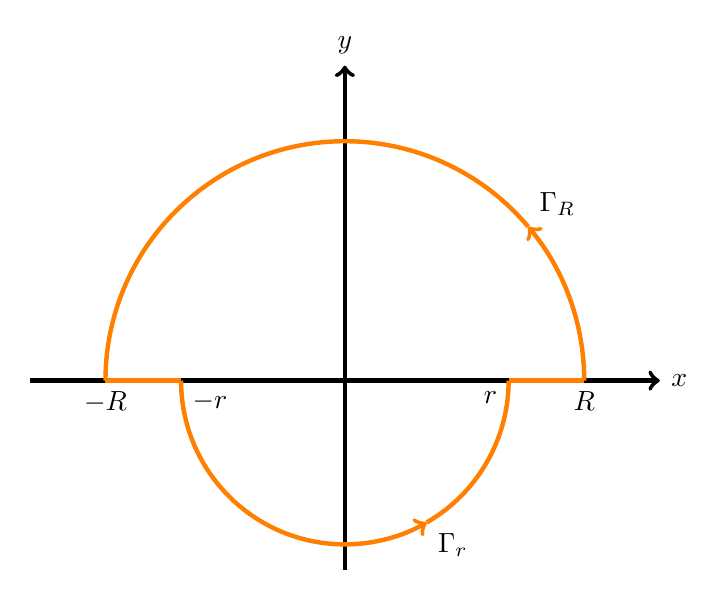
\begin{tikzpicture}[scale=.8]
\draw[ultra thick,->]
	(-5,0)--(5,0)node[right]{\(x\)};
\draw[ultra thick,->]
	(0,-3)--(0,5)node[above]{\(y\)};
\pgfmathsetmacro{\R}{3.8}
\pgfmathsetmacro{\r}{2.6}
\begin{scope}[ultra thick,orange]
\draw (-\R,0)node[below,black]{\(-R\)}--(-\r,0)node[below right,black]{\(-r\)} (\r,0)node[below left,black]{\(r\)}--(\R,0)node[below,black]{\(R\)};
\draw[->] (-\r,0)arc[start angle=180,end angle=300,radius=\r]node[below right,black]{\(\Gamma_r\)};
\draw (\r,0)arc[start angle=0,end angle=-60,radius=\r];
\draw[->] (\R,0)arc[start angle=0,end angle=40,radius=\R]node[above right,black]{\(\Gamma_R\)};
\draw (-\R,0)arc[start angle=180,end angle=40,radius=\R];
\end{scope}
\end{tikzpicture}
\caption{狄利克雷积分的辅助积分路径}
\label{figure:留数定理.狄利克雷积分的辅助积分路径}
\end{figure}

设\(f(z) = \frac{1}{z}\),\(F(z) = \frac{e^{\iu z}}{z}\),则\(F(z)\)中的\(z\)取实值\(x\)时,其虚部即所求实积分的被积函数.
因为\(z=0\)是\(F(z)\)的一阶极点,它处在\cref{theorem:留数定理.利用留数定理计算实积分3} 中对辅助函数\(F(z) = e^{\iu\alpha z} f(z)\)的围线积分的积分路径上,所以不能直接应用\cref{equation:留数定理.利用留数定理计算实积分3.1}.
我们改为考虑取\cref{figure:留数定理.狄利克雷积分的辅助积分路径} 所示的积分路径来绕开奇点,再应用\hyperref[theorem:留数定理.柯西留数定理]{留数定理},得\[
\begin{split}
&\hspace{-20pt}\int_r^R F(x) \dd{x}
+ \int_{\Gamma_R} F(z) \dd{z}
+ \int_{-R}^{-r} F(x) \dd{x}
+ \int_{\Gamma_r} F(z) \dd{z} \\
&= 2\pi\iu \Res_{z=0} F(z)
= 2\pi\iu \Res_{z=0} \frac{e^{\iu z}}{z}
= 2\pi\iu,
\end{split}
\]又由\hyperref[theorem:留数定理.计算积分路径上没有奇点的无穷限积分.引理2]{若尔当引理},有\[
\lim_{R\to+\infty} \int_{\Gamma_R} F(z) \dd{z} = 0.
\]在\(\Gamma_r\)上的积分,根据\(\lim_{z\to0} z F(z) = 1\),以及\cref{theorem:留数定理.计算积分路径上没有奇点的无穷限积分.引理1},有\[
\lim_{r\to0} \int_{\Gamma_r} F(z) \dd{z} = \pi\iu.
\]又因\[
\int_{-R}^{-r} F(x) \dd{x}
= \int_{-R}^{-r} \frac{e^{\iu x}}{x} \dd{x}
= -\int_r^R \frac{e^{-\iu x}}{x} \dd{x},
\]所以\[
\int_r^R \frac{e^{\iu x} - e^{-\iu x}}{x} \dd{x}
+ \int_{\Gamma_R} F(z) \dd{z}
+ \int_{\Gamma_r} F(z) \dd{z}
= 2\pi\iu,
\]即\[
2\iu \int_r^R \frac{\sin x}{x} \dd{x}
+ \int_{\Gamma_R} F(z) \dd{z}
+ \int_{\Gamma_r} F(z) \dd{z}
= 2\pi\iu.
\]令\(r\to0, R\to+\infty\),即得\(\int_0^{+\infty} \frac{\sin x}{x} \dd{x} = \frac{\pi}{2}\).
\end{solution}
\end{example}

\subsection{其他情形}
还有一些无穷限积分,不满足\cref{theorem:留数定理.利用留数定理计算实积分2,theorem:留数定理.利用留数定理计算实积分3} 的条件,不能简单地引用这些定理来进行计算,但我们可以借鉴这些定理的证明思路:构造围线积分,应用留数定理(或作为其特殊情形的柯西积分定理),估计或计算辅助函数在辅助积分路径上的积分,再取极限,进而得到我们所要计算的广义积分.

\begin{example}
计算泊松积分\[
I = \int_0^{+\infty} e^{-ax^2} \cos bx \dd{x} \quad(a>0).
\]
\begin{solution}
若\(b=0\),则令\(t=\sqrt{a}x\)之后,\[
I = \int_0^{+\infty} e^{-ax^2} \dd{x}
= \frac{1}{\sqrt{a}} \int_0^{+\infty} e^{-t^2} \dd{t}
= \frac{1}{\sqrt{a}} \cdot \frac{\sqrt{\pi}}{2}
= \frac{1}{2} \sqrt{\frac{\pi}{a}}.
\eqno(1)
\]

若\(b\neq0\),因为\(\cos bx\)是偶函数,所以只需考虑\(b > 0\)的情形.
首先取辅助函数\(F_1(z) = e^{-az^2} e^{\iu bz}\),则\begin{align*}
I &= \frac{1}{2} \Re \int_{-\infty}^{+\infty} e^{-(ax^2+\iu bx)} \dd{x} \\
&= \frac{1}{2} \Re\left\{ e^{-\frac{b^2}{4a}} \int_{-\infty}^{+\infty} e^{-a\left(x+\frac{b}{2a}\iu\right)^2} \dd{x} \right\} \\
&= \frac{1}{2} e^{-\frac{b^2}{4a}} \int_{-\infty+\frac{b}{2a}\iu}^{+\infty+\frac{b}{2a}\iu} e^{-az^2} \dd{z}.
\tag2
\end{align*}

又由(1)式可知\[
\int_{-\infty}^{+\infty} e^{-ax^2} \dd{x}
= \sqrt{\frac{\pi}{a}}.
\eqno(3)
\]

\begin{figure}[ht]
\centering
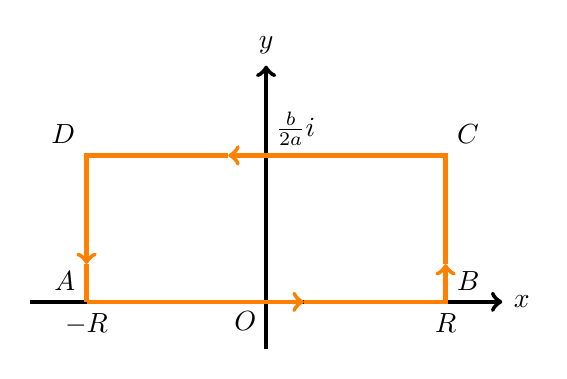
\begin{tikzpicture}[scale=.6]
\draw[ultra thick,->]
	(-5,0)--(5,0)node[right]{\(x\)};
\draw[ultra thick,->]
	(0,-1)--(0,5)node[above]{\(y\)};
\pgfmathsetmacro{\R}{3.8}
\pgfmathsetmacro{\b}{3.1}
\begin{scope}[ultra thick,orange]
\draw[->] (-\R,0)node[above left,black]{\(A\)}node[below,black]{\(-R\)}--(.8,0);
\draw[->] (.8,0)--(\R,0)node[above right,black]{\(B\)}node[below,black]{\(R\)}--(\R,.8);
\draw[->] (\R,.8)--(\R,\b)node[above right,black]{\(C\)}--(-.8,\b);
\draw[->] (-.8,\b)--(-\R,\b)node[above left,black]{\(D\)}--(-\R,.8);
\draw (-\R,.8)--(-\R,0);
\end{scope}
\draw (0,\b)node[above right]{\(\frac{b}{2a}i\)};
\draw (0,0)node[below left]{\(O\)};
\end{tikzpicture}
\caption{泊松积分的辅助积分路径}
\label{figure:留数定理.泊松积分的辅助积分路径}
\end{figure}
取辅助函数\(F(z) = e^{-az^2}\),再取\cref{figure:留数定理.泊松积分的辅助积分路径} 所示的积分路径\(\Gamma = AB+BC+CD+DA\).
由\hyperref[theorem:解析函数的积分表示.柯西积分定理]{柯西积分定理}得\[
\int_\Gamma e^{-az^2} \dd{z} = 0.
\eqno(4)
\]

比较(2)式与(4)式,得到\[
\begin{split}
I &\xlongequal{\rm(2)} \frac{1}{2} e^{-\frac{b^2}{4a}} \Re\left[\lim_{R\to+\infty} \left( \int_{DC} e^{-az^2} \dd{z} \right)\right] \\
&\xlongequal{\rm(4)} \frac{1}{2} e^{-\frac{b^2}{4a}} \Re\left[\lim_{R\to+\infty} \left( \int_{AB} + \int_{BC} + \int_{DA}\right) e^{-az^2} \dd{z}\right].
\end{split}
\]
在线段\(BC\)及\(DA\)上,\(z=\pm R+\iu y\ (0 \leq y \leq \frac{b}{2a})\),\[
\abs{e^{-az^2}}
= e^{-a(R^2-y^2)}
\leq e^{\frac{b^2}{4a}} \cdot e^{-aR^2},
\]故\[
\lim_{R\to+\infty} \int_{BC} e^{-az^2} \dd{z} = 0,
\qquad
\lim_{R\to+\infty} \int_{DA} e^{-az^2} \dd{z} = 0.
\]最后得到\[
I = \frac{1}{2} e^{-\frac{b^2}{4a}} \Re\left[ \lim_{R\to+\infty} \int_{AB} e^{-az^2} \dd{z} \right]
\xlongequal{\rm(3)} \frac{1}{2} \sqrt{\frac{\pi}{a}} e^{-\frac{b^2}{4a}},
\]即\begin{equation}\label{equation:留数定理.泊松积分}
\int_0^{+\infty} e^{-ax^2} \cos bx \dd{x}
= \frac{1}{2} \sqrt{\frac{\pi}{a}} e^{-\frac{b^2}{4a}}
\quad(a>0).
\end{equation}
\end{solution}
\end{example}

\begin{example}
计算菲涅耳积分\[
\int_0^{+\infty} \cos x^2 \dd{x}
\quad\text{及}\quad
\int_0^{+\infty} \sin x^2 \dd{x}.
\]
\begin{solution}
\begin{figure}[ht]
\centering
\begin{tikzpicture}
\draw[thick,->]
	(-.1,0)--(4.3,0)node[right]{\(x\)};
\pgfmathsetmacro{\R}{4}
\pgfmathsetmacro{\bx}{\R*cos(45)}
\pgfmathsetmacro{\by}{\R*sin(45)}
\coordinate (O) at (0,0);
\coordinate (A) at (\R,0);
\coordinate (B) at (\bx,\by);
\draw pic["\(\frac{\pi}{4}\)",draw=blue,-,angle eccentricity=1.5,angle radius=8mm]{angle=A--O--B};
\begin{scope}[ultra thick,orange]
\draw[->] (O)--(3,0)node[below,black]{\(\Gamma_R\)};
\draw (3,0)--(A)node[below,black]{\(R\)}arc[start angle=0,end angle=45,radius=\R]--(O);
\end{scope}
\draw (O)node[below left]{\(O\)};
\end{tikzpicture}
\caption{菲涅耳积分的辅助积分路径}
\label{figure:留数定理.菲涅耳积分的辅助积分路径}
\end{figure}

选取辅助函数\(F(z) = e^{-z^2}\),并取如\cref{figure:留数定理.菲涅耳积分的辅助积分路径} 所示的辅助积分路径\(C_R\),则由柯西积分定理有\[
\int_{C_R} e^{-z^2} \dd{z}
= \int_0^R e^{-x^2} \dd{x}
+ \int_{\Gamma_R} e^{-z^2} \dd{z}
+ \int_R^0 \exp[-\left(x e^{\frac{1}{4}\pi\iu}\right)^2] \dd(x e^{\frac{1}{4}\pi\iu})
= 0.
\]
在\(\Gamma_R\)上,\(z = R e^{\iu\theta}\ (0\leq\theta\leq\frac{\pi}{4})\),\(z^2 = R^2 e^{\iu2\theta}\).
利用\hyperref[equation:微分中值定理.若尔当不等式]{若尔当不等式}\[
0\leq\theta\leq\frac{\pi}{2}
\implies
\sin\theta\geq\frac{2\theta}{\pi},
\]可得\begin{align*}
\abs{\int_{\Gamma_R} e^{-z^2} \dd{z}}
&\leq
\int_0^{\frac{\pi}{4}} \exp(-R^2 \cos2\theta) R\dd{\theta} \\
&\xlongequal{2\theta=\frac{\pi}{2}-\phi}
\frac{R}{2} \int_0^{\frac{\pi}{2}} \exp(-R^2 \sin\phi) \dd{\phi} \\
&\leq
\frac{R}{2} \int_0^{\frac{\pi}{2}} \exp(-\frac{2R^2}{\pi}\phi) \dd{\phi} \\
&= \frac{\pi}{4R} (1-e^{-R^2})
\to0\quad(R\to+\infty).
\end{align*}
所以\[
\lim_{R\to+\infty} \left[
\int_0^R \exp(-x^2) \dd{x}
+ \int_R^0 \exp(-x^2 e^{\frac{1}{2}\pi\iu}) \cdot \exp(\frac{1}{4}\pi\iu) \dd{x}
\right] = 0,
\]\[
\int_0^{+\infty} \exp(-x^2) \dd{x} - \exp(\frac{1}{4}\pi\iu) \int_0^{+\infty} (\cos x^2 - \iu \sin x^2) \dd{x} = 0.
\]又因为\(\int_0^{+\infty} e^{-x^2} \dd{x} = \frac{\sqrt{\pi}}{2}\),故\[
\int_0^{+\infty} \cos x^2 \dd{x}
- \iu \int_0^{+\infty} \sin x^2 \dd{x}
= \frac{\sqrt{\pi}}{2} \exp(-\frac{1}{4}\pi\iu)
= \frac{\sqrt{\pi}}{2} \left(\cos\frac{\pi}{4} - \iu \sin\frac{\pi}{4}\right).
\]比较实部、虚部得\begin{equation}\label{equation:留数定理.菲涅耳积分}
\int_0^{+\infty} \cos x^2 \dd{x}
= \int_0^{+\infty} \sin x^2 \dd{x}
= \frac{1}{2} \sqrt{\frac{\pi}{2}}.
\end{equation}
\end{solution}
\end{example}

从前面的几个模式可见,利用留数定理计算实积分,难点和关键在于选择恰当的辅助函数以及一条相应的辅助积分路径.
除了一些标准模式外,辅助函数尤其是辅助积分路径的选择很不规则.
一般来说,辅助函数\(F(z)\)总要选得使\(z\)取实值\(x\)时,\(F(x)\)等于实积分的被积函数\(f(x)\),或\(\Re{F(z)} = f(x)\),或\(\Im{F(z)} = f(x)\).
辅助积分路径的选择原则是:使添加的积分路径上的复积分能够通过一定的办法估计或计算出来,或者能够转化为原来要计算的实积分.
但具体选择时,形状则是多种多样的,有半圆周围线、长方形围线、扇形围线、三角形围线等等.
此外,围线上有奇点时还要绕开奇点.

\subsection{计算多值函数的积分}
在计算某些广义实积分时,需要选择的辅助函数有时是多值函数,这时必须适当割破复平面,使多值函数能够分出单值解析分支,才能应用柯西留数定理或柯西积分定理,进而求出所给广义实积分的值.

\subsubsection{计算\texorpdfstring{\(\int_0^{+\infty} f(x) \ln x \dd{x}\)型}{含有对数函数的}无穷限积分}
利用留数定理计算这种形式的积分时,其辅助函数的选择就避不开多值函数\(\Ln z\).
为了使\(z\)取实值时\(\Ln z\)取实积分被积函数中的\(\ln x\),我们必须割破\(z\)平面,使\(\Ln z\)能够分出单值的解析分支,并取其中的主值\(\ln z\).
在前面谈到将\(\Ln z\)分出单值解析分支时,我们总是从原点起沿负实轴割破\(z\)平面.
其实从原点起沿正实轴割破\(z\)平面也能将\(\Ln z\)分出单值解析分支.
在下面的定理,限制\(0 < \Im \ln z = \arg z < 2\pi\),也就意味着是沿正实轴割破\(z\)平面的.

\begin{theorem}\label{theorem:留数定理.利用留数定理计算实积分4}
若函数\(f(z)\)在扩充复平面\(\mathbb{C}_\infty\)上只有有限个孤立奇点\(\AutoTuple{a}{n}\),且这些奇点不在包括原点的正实轴上,\(f(z)\)在实轴上取实值,此外\(z=\infty\)是\(f(z)\)的\(m\ (m\geq2)\)阶零点,则\begin{equation}\label{equation:留数定理.利用留数定理计算实积分4.1}
\int_0^{+\infty} f(x) \ln x \dd{x}
= -\frac{1}{2} \Re{ \sum_{k=1}^n \Res_{z=a_k} \left[ f(z) \ln^2 z \right] },
\end{equation}
其中\(\ln z\)是复对数函数\(\Ln z\)的主值,\(0<\Im \ln z<2\pi\).

特别地,若\(f(x) = \frac{P_n(x)}{Q_m(x)}\)是实系数的有理分式函数,分母多像是\(Q_m(x)\)的零点不在包括原点的正实轴上,且\(Q_m(x)\)的次数\(m\)至少比\(P_n(x)\)的次数\(n\)大\(2\),即\(m-n\geq2\),则\cref{equation:留数定理.利用留数定理计算实积分4.1} 成立.
\begin{proof}
\begin{figure}[ht]
\centering
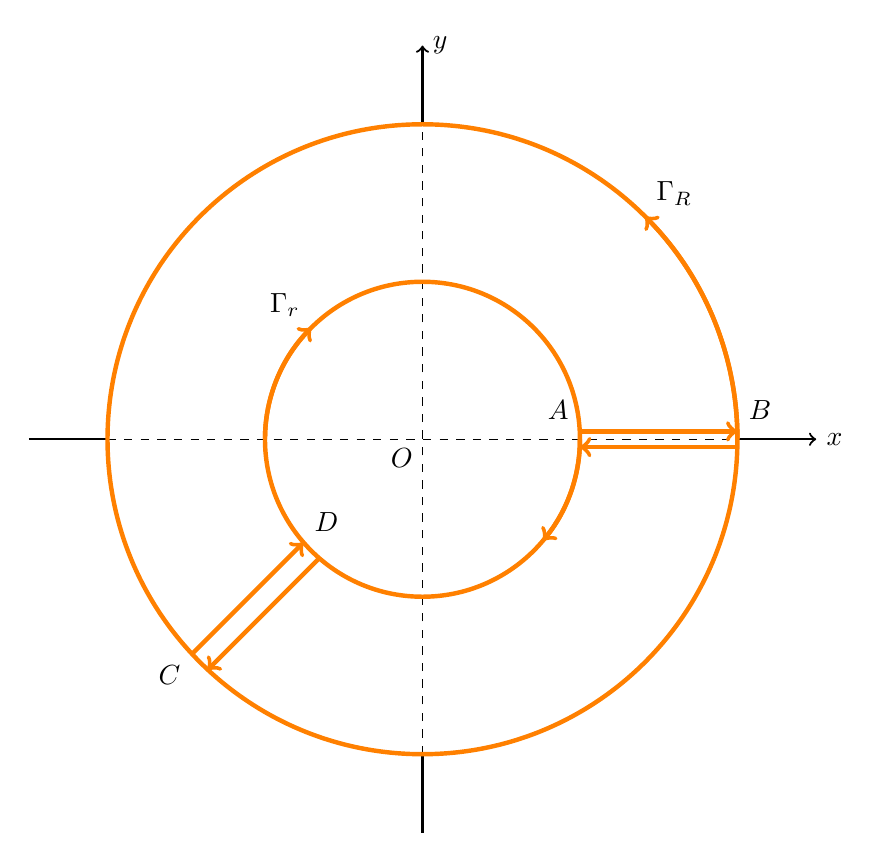
\begin{tikzpicture}
\pgfmathsetmacro{\R}{4}
\pgfmathsetmacro{\r}{2}
\pgfmathsetmacro{\cx}{\R*cos(225)}
\pgfmathsetmacro{\cy}{\R*sin(225)}
\pgfmathsetmacro{\dx}{\r*cos(225)}
\pgfmathsetmacro{\dy}{\r*sin(225)}
\draw[thick,->]
	(-5,0)--(-\R,0) (\R,0)--(5,0)node[right]{\(x\)};
\draw[thick,->]
	(0,-5)--(0,-\R) (0,\R)--(0,5)node[right]{\(y\)};
\draw[dashed] (-\R,0)--(\R,0) (0,-\R)--(0,\R);
\coordinate (O) at (0,0);
\coordinate (A) at (\r,.1);
\coordinate (B) at (\R,.1);
\begin{scope}[ultra thick,orange]
\draw (O)circle(\R)circle(\r);
\begin{scope}[->]
\draw (A)node[above left,black]{\(A\)}--(B)node[above right,black]{\(B\)};
\draw (\R,-.1)--(\r,-.1);
\draw (\R,0)arc[start angle=0,end angle=45,radius=\R]node[above right,black]{\(\Gamma_R\)};
\draw (-\r,0)arc[start angle=180,end angle=135,radius=\r]node[above left,black]{\(\Gamma_r\)};
\draw (\r,0)arc[start angle=0,end angle=-40,radius=\r];
\draw (\cx-.1,\cy+.1)node[below left,black]{\(C\)}--(\dx-.1,\dy+.1)node[above right,black]{\(D\)};
\draw (\dx+.1,\dy-.1)--(\cx+.1,\cy-.1);
\end{scope}
\end{scope}
\draw (O)node[below left]{\(O\)};
\end{tikzpicture}
\caption{}
\label{figure:留数定理.利用留数定理计算实积分4的辅助积分路径1}
\end{figure}
取辅助围线如\cref{figure:留数定理.利用留数定理计算实积分4的辅助积分路径1} 所示的\[
\Gamma = AB \cup \Gamma_R \cup BA \cup \Gamma_r^-,
\]其中\(AB\)沿支割线上岸,\(BA\)沿支割线下岸\footnote{曲线\(\Gamma\)虽不是简单闭曲线,但用连接内外圆周的直线段\(CD\)可将\(\Gamma\)变为两条简单闭曲线,在它们所围的两个区域内应用留数定理,由于在线段\(CD\)上来回积分两次,其和为零,所以可在\(\Gamma\)所围区域内应用留数定理.}.
取辅助函数\[
F(z) = f(z) \ln^2 z,
\]其中\(\ln z\)是\(\Ln z\)的主值,而\(0<\Im\ln z<2\pi\).
\(F(z)\)在\(\Gamma\)的“内部”(除\(\AutoTuple{a}{n}\))解析,且连续到边界\(\Gamma\)(在\(AB,BA\)上分别是从上、下半平面连续到\(AB,BA\)).
由留数定理,得\[
\left(\int_{AB}+\int_{\Gamma_R}+\int_{BA}+\int_{\Gamma_r^-}\right) F(z) \dd{z}
= 2\pi\iu \sum_{k=1}^n \Res_{z=a_k} F(z).
\]

在线段\(AB\)上,\(z=x\),\(F(z) = f(x) \ln^2 x\),因此\[
\int_{AB} F(z) \dd{z}
= \int_r^R f(x) \ln^2 x \dd{x}.
\]

在线段\(BA\)上,\(z = x e^{2\pi\iu}\),\(F(z) = f(x) (\ln x + 2\pi\iu)^2\),所以\[
\int_{BA} F(z) \dd{z}
= -\int_r^R f(x) (\ln x + 2\pi\iu)^2 \dd{x}.
\]

在\(\Gamma_R\)上,\(z = R e^{\iu\theta}\ (0\leq\theta\leq2\pi)\),\[
\abs{\ln z}^2 = \ln^2 R + \theta^2 \leq 2 \ln^2 R.
\]

点\(z=\infty\)是\(f(z)\)的\(m\)阶零点.
当\(R\)充分大时,\(\abs{f(z)} \leq M/R^m\ (M>0)\).
于是,\[
\abs{\int_{\Gamma_R} F(z) \dd{z}}
\leq \frac{M}{R^m} \cdot 2 \ln^2 R \cdot 2\pi R
= \frac{4M \ln^2 R}{R^{m-1}} \to 0 \quad(R\to+\infty).
\]

在\(\Gamma_r\)上,\(z = r e^{\iu\theta}\ (0\leq\theta\leq2\pi)\),从而\[
\abs{\ln z}^2 = \ln^2 r + \theta^2
\leq 2 \ln^2 \frac{1}{r}.
\]

\(f(z)\)在点\(z=0\)的邻域内有界,所以\[
\abs{F(z)} \leq 2M_1 \ln^2 \frac{1}{r},
\]\[
\abs{\int_{\Gamma_r} F(z) \dd{z}}
\leq 4\pi M_1 r \ln^2 \frac{1}{r}
\to 0 \quad(r\to0^+).
\]

于是,\(r\to0^+, R\to+\infty\)时,有\[
\int_0^{+\infty} f(x) \ln^2 x \dd{x}
- \int_0^{+\infty} f(x) (\ln x + 2\pi\iu)^2 \dd{x}
= 2\pi\iu \sum_{k=1}^n \Res_{z=a_k} F(z),
\]\[
-4\pi\iu \int_0^{+\infty} f(x) \ln x \dd{x}
+ 4\pi^2 \int_0^{+\infty} f(x) \dd{x}
= 2\pi\iu \sum_{k=1}^n \Res_{z=a_k} F(z).
\]
在上式两边取虚部,即得\begin{equation}\label{equation:留数定理.利用留数定理计算实积分4.2}
\int_0^{+\infty} f(x) \ln x \dd{x}
= -\frac{1}{2} \Re{ \sum_{k=1}^n \Res_{z=a_k} \left[ f(z) \ln^2 z \right] };
\end{equation}
取实部,即得\begin{equation}\label{equation:留数定理.利用留数定理计算实积分4.3}
\int_0^{+\infty} f(x) \dd{x}
= -\frac{1}{2\pi} \Im{ \sum_{k=1}^n \Res_{z=a_k} \left[ f(z) \ln^2 z \right] }.
\end{equation}
\end{proof}
\end{theorem}

\begin{figure}[ht]
\centering
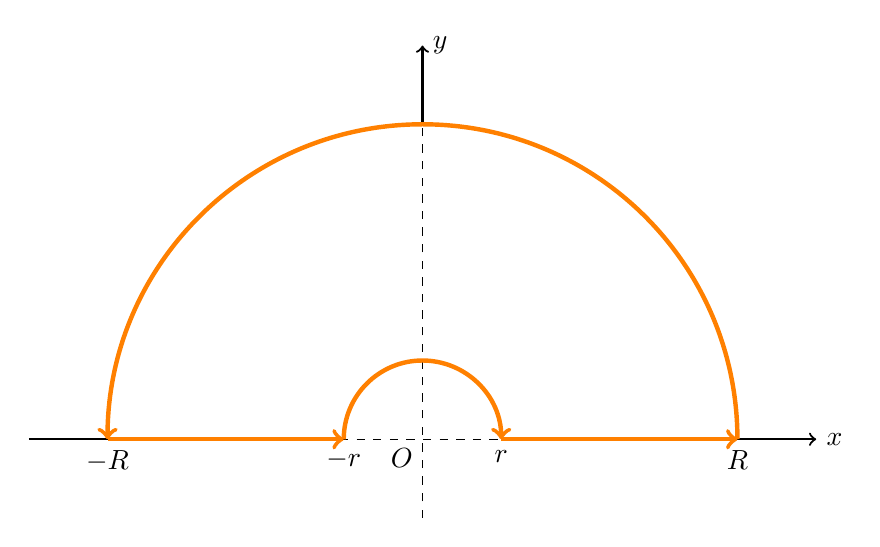
\begin{tikzpicture}
\pgfmathsetmacro{\R}{4}
\pgfmathsetmacro{\r}{1}
\draw[thick,->]
	(-5,0)--(-\R,0) (\R,0)--(5,0)node[right]{\(x\)};
\draw[thick,->]
	(0,\R)--(0,5)node[right]{\(y\)};
\draw[dashed] (-\R,0)--(\R,0) (0,-1)--(0,\R);
\coordinate (O) at (0,0);
\begin{scope}[ultra thick,orange]
\begin{scope}[->]
\draw (\r,0)node[below,black]{\(r\)}--(\R,0)node[below,black]{\(R\)};
\draw (\R,0)arc[start angle=0,end angle=180,radius=\R];
\draw (-\R,0)node[below,black]{\(-R\)}--(-\r,0)node[below,black]{\(-r\)};
\draw (-\r,0)arc[start angle=180,end angle=0,radius=\r];
\end{scope}
\end{scope}
\draw (O)node[below left]{\(O\)};
\end{tikzpicture}
\caption{}
\label{figure:留数定理.利用留数定理计算实积分4的辅助积分路径2}
\end{figure}
若\(f(x)\)是偶函数,\(f(z)\)在上半平面\(\Im z > 0\)内除去有限多个孤立奇点\(\AutoTuple{a}{n}\)外是解析的,在\(\Im z \geq 0\)上除去\(\AutoTuple{a}{n}\)外连续,且\[
\exists M>0,\forall m\geq2, \exists N>0 \left[
\abs{z}>N
\implies
\abs{f(z)}\leq\frac{M}{\abs{z}^m}
\right],
\]则令\(F(z) = f(z) \ln z\),并取如\cref{figure:留数定理.利用留数定理计算实积分4的辅助积分路径2} 所示的辅助围线,则有\begin{gather}
\int_0^{+\infty} f(x) \ln x \dd{x}
= -\pi \Im{ \sum_{k=1}^n \Res_{z=a_k}[ f(z) \ln z ] }, \label{equation:留数定理.利用留数定理计算实积分4.4} \\
\int_0^{+\infty} f(x) \dd{x}
= 2 \Re{ \sum_{k=1}^n \Res_{z=a_k}[ f(z) \ln z ] }. \label{equation:留数定理.利用留数定理计算实积分4.5}
\end{gather}

\begin{example}
计算积分\[
I = \int_0^{+\infty} \frac{\ln x}{(1+x^2)^2} \dd{x}.
\]
\begin{solution}
因为函数\(f(x) = \frac{1}{(1+x^2)^2}\)是偶函数,也可用\cref{equation:留数定理.利用留数定理计算实积分4.4} 计算这个积分:\begin{align*}
\Res_{z=\iu} \frac{\ln z}{(1+z^2)^2}
&= \eval{\left\{ \dv{z} \left[ \frac{\ln z}{(z+\iu)^2} \right] \right\}}_{z=\iu} \\
&= \eval{\left\{ \frac{1}{z(z+\iu)^2} - \frac{2 \ln z}{(z+\iu)^3} \right\}}_{z=\iu} \\
&= \frac{\pi}{8} + \frac{\iu}{4},
\end{align*}\[
\int_0^{+\infty} \frac{\ln x}{(1+x^2)^2} \dd{z}
= -\pi \Im\left(\frac{\pi}{8}+\frac{\iu}{4}\right) = -\frac{\pi}{4}.
\]
\end{solution}
\end{example}

\subsubsection{计算\texorpdfstring{\(\int_0^{+\infty} f(x) x^{p-1} \dd{x}\ (0<p<1)\)型}{含有幂函数的}无穷限积分}
\begin{theorem}\label{theorem:留数定理.利用留数定理计算实积分5}
若函数\(f(z)\)在扩充复平面\(\mathbb{C}_\infty\)上除去有限个点\(\AutoTuple{a}{n}\)外解析,且\(\AutoTuple{a}{n}\)不在包括原点的正实轴上,点\(z=\infty\)是\(f(z)\)的\(m\ (m\geq1)\)阶零点,则\begin{equation}\label{equation:留数定理.利用留数定理计算实积分5.1}
\int_0^{+\infty} f(x) x^{p-1} \dd{x}
= \frac{2\pi\iu}{1-e^{2\pi p\iu}} \sum_{k=1}^n \Res_{z=a_k}[f(z) z^{p-1}],
\end{equation}
其中\(z^{p-1} = e^{(p-1) \ln z}\ (0<\Im\ln z = \arg z<2\pi)\).

特别地,若\(f(x) = \frac{P_n(x)}{Q_m(x)}\)是有理分式函数,\(Q_m(x)\)在包括原点的正实轴上没有零点,分母多项式\(Q_m(x)\)的次数\(m\)比分子多项式\(P_n(x)\)的次数\(n\)至少大\(1\),即\(m-n\geq1\),则\cref{equation:留数定理.利用留数定理计算实积分5.1} 成立.
\begin{proof}
取辅助函数\(F(z) = z^{p-1} f(z) = e^{(p-1)\ln z} f(z)\),其中\[
\ln z = \ln\abs{z} + \iu\arg z \quad(0<\arg z<2\pi).
\]
取辅助围线\(C\)如\cref{figure:留数定理.利用留数定理计算实积分4的辅助积分路径1} 所示,\(C=AB+\Gamma_R+BA+\Gamma_r^-\).
由留数定理,得\begin{align*}
&\hspace{-20pt}\int_r^R e^{(p-1)\ln x} f(x) \dd{x}
+ \int_{\Gamma_R} F(z) \dd{z}
+ \int_R^r e^{(p-1)(\ln x+2\pi\iu)} f(x) \dd{x}
+ \int_{\Gamma_r^-} F(z) \dd{z} \\
&= 2\pi\iu \sum_{k=1}^n \Res_{z=a_k} F(z),
\end{align*}整理得\[
(1-e^{2\pi p\iu}) \int_r^R x^{p-1} f(x) \dd{x}
+ \left(\int_{\Gamma_r^-}+\int_{\Gamma_R}\right) F(z) \dd{z}
= 2\pi\iu \sum_{k=1}^n \Res_{z=a_k} F(z).
\eqno(1)
\]

在\(\Gamma_r\)上有\begin{align*}
\abs{\int_{\Gamma_r^-} F(z) \dd{z}}
&= \abs{\int_{\Gamma_r^-} e^{(p-1)(\ln r + \iu\arg z)} f(z) \dd{z}} \\
&= r^{p-1} \max_{z\in\Gamma_r} \abs{f(z)} \cdot 2\pi r \\
&= 2\pi r^p \max_{z\in\Gamma_r} \abs{f(z)} \to0\quad(r\to0),
\end{align*}
同理有\[
\abs{\int_{\Gamma_R} F(z) \dd{z}}
\leq 2\pi R^p \max_{z\in\Gamma_R} \abs{f(z)}.
\]

由于\(z=\infty\)为\(f(z)\)的\(m\)阶零点,当\(R\)充分大时,在\(\Gamma_R\)上\(\abs{f(z)}<M/R^m\),\(M\)是正常数,\(m\geq1\),所以\[
\abs{\int_{\Gamma_R} F(z) \dd{z}}
\leq \frac{2\pi M}{R^{m-p}} \to0\quad(R\to+\infty).
\]在(1)式中令\(r\to0^+,R\to+\infty\),得到\[
(1-e^{2\pi p\iu}) \int_0^{+\infty} x^{p-1} f(x) \dd{x}
= 2\pi\iu \sum_{k=1}^n \Res_{z=a_k} F(z).
\]于是得到\cref{equation:留数定理.利用留数定理计算实积分5.1} 或者\begin{equation}\label{equation:留数定理.利用留数定理计算实积分5.2}
\int_0^{+\infty} x^{p-1} f(x) \dd{x}
= -\frac{\pi}{e^{p\pi\iu} \sin p\pi} \sum_{k=1}^n \Res_{z=a_k}[z^{p-1} f(z)].
\end{equation}
注:关于\(p\),只要假定\(0<p<m\),且\(p\notin\mathbb{Z}\),则\cref{equation:留数定理.利用留数定理计算实积分5.1} 成立.
若\(f(x)\)是偶函数,仍可采用\cref{figure:留数定理.利用留数定理计算实积分4的辅助积分路径2} 所示的积分路径,得出相应的结果.
\end{proof}
\end{theorem}

\begin{example}
计算欧拉积分\[
I = \int_0^{+\infty} \frac{x^{p-1}}{1+x} \dd{x} \quad(0<p<1).
\]
\begin{solution}
这里\(f(x) = \frac{1}{1+x}\)满足\cref{theorem:留数定理.利用留数定理计算实积分5} 的条件.
点\(z=-1\)是\(f(z) = \frac{1}{1+z}\)的一阶极点,\(z=\infty\)是\(f(z)\)的一阶零点.
\(F(z) = z^{p-1} \frac{1}{1+z}\)在点\(z=-1\)处的留数\[
\Res_{z=-1} F(z)
= \lim_{z\to-1} (z+1) \frac{z^{p-1}}{1+z}
= \lim_{\substack{\abs{z}\to1 \\ \theta\to\pi}} \exp[(p-1)(\ln\abs{z}+\iu\theta)]
= e^{(p-1)\pi\iu}
= -e^{p\pi\iu}.
\]应用\cref{equation:留数定理.利用留数定理计算实积分5.2} 即有\begin{equation}
\int_0^{+\infty} \frac{x^{p-1}}{1+x} \dd{x} = \frac{\pi}{\sin p\pi}.
\end{equation}
\end{solution}
\end{example}

\begin{example}%https://www.bilibili.com/video/BV1Vb4y1Y7Sn/
计算定积分\[
\int_0^1 \frac{\ln x}{x^2-x-1} \dd{x}.
\]
\begin{solution}
首先求出所求积分\(I = \int_0^1 \frac{\ln x}{x^2-x-1} \dd{x}\)的奇点,即方程\(x^2-x-1=0\)的根,得\[
x_1 = \frac{1-\sqrt{5}}{2}, \qquad
x_2 = \frac{1+\sqrt{5}}{2}.
\]

取割线\(L = \Set{x \given x\in[0,1]} \cup \Set{1+\iu y \given y\in[0,+\infty)}\).
我们利用复对数函数\(\Ln z\)作为辅助函数,并令\(\Ln\frac{1}{2} = \ln\frac{1}{2}\).
以\(L_1,L_2\)分别表示射线\(\Set{1+\iu y \given y\in[0,+\infty)}\)的右侧和左侧,方向向上;
以\(L_3,L_4\)分别表示线段\(\Set{x \given x\in[0,1]}\)的上侧和下侧,方向向右.

根据留数定理\[
\left(\int_{L_2} - \int_{L_1} - \int_{L_4} + \int_{L_3}\right) \frac{\Ln^2 z}{z^2-z-1} \dd{z}
= 2\pi\iu \left[\Res_{z=x_1} f(z) + \Res_{z=x_2} f(z)\right].
\eqno(1)
\]

在\(L_2\)上,\(z=1+\iu y\),从而\(\abs{z}=\sqrt{1+y^2},
\arg z = \arctan y,
\dd{z} = \iu \dd{y}\),\[
\int_{L_2} \frac{\Ln^2 z}{z^2-z-1} \dd{z}
= \int_0^{+\infty} \frac{\left(\ln\sqrt{1+x^2} + \iu \arctan x\right)^2}{-x^2+\iu x-1} \iu \dd{x}.
\]

在\(L_1\)上,因为它是下沿,所以\[
\Ln^2 z = \left(\ln\sqrt{1+x^2} + \iu \arctan x + 2\pi\iu\right)^2,
\]那么\[
\int_{L_1} \frac{\Ln^2 z}{z^2-z-1} \dd{z}
= \int_0^{+\infty} \frac{\left(\ln\sqrt{1+x^2} + \iu \arctan x + 2\pi\iu\right)^2}{-x^2+\iu x-1} \iu \dd{x}.
\]

在\(L_4\)上,\(z=x\),因为它是下沿,所以\[
\int_{L_4} \frac{\Ln^2 z}{z^2-z-1} \dd{z}
= \int_0^1 \frac{\left(\ln x + 2\pi\iu\right)^2}{x^2-x-1} \dd{x}.
\]

在\(L_3\)上,\(z=x\),\[
\int_{L_3} \frac{\Ln^2 z}{z^2-z-1} \dd{z}
= \int_0^1 \frac{\ln^2 x}{x^2-x-1} \dd{x}.
\]

因为\[
\Res_{z=x_1} f(z)
= \frac{\left(\ln\abs{x_1} + \pi\iu\right)^2}{x_1 - x_2},
\qquad
\Res_{z=x_2} f(z)
= \frac{\left(\ln\abs{x_2} + 2\pi\iu\right)^2}{x_2 - x_1},
\]且(1)式左侧可化简得\begin{align*}
2\pi \left(
\int_0^{+\infty} \frac{2\ln\sqrt{1+x^2} + 2\iu \arctan x + 2\pi\iu}{-x^2+\iu x-1} \dd{x}
+ \int_0^1 \frac{-2\iu \ln x + 2\pi}{x^2-x-1} \dd{x}
\right),
\end{align*}
那么对(1)式两边取虚部并同除以\((-2\pi)\)可得\[
-\Im \int_0^{+\infty} \frac{2\ln\sqrt{1+x^2} + 2\iu \arctan x + 2\pi\iu}{-x^2+\iu x-1} \dd{x}
+ 2I = \frac{3\pi^2}{\sqrt{5}}.
\]

进行分母有理化,有\begin{align*}
&-\Im \int_0^{+\infty} \frac{2\ln\sqrt{1+x^2} + 2\iu \arctan x + 2\pi\iu}{-x^2+\iu x-1} \dd{x} \\
&= -\Im \int_0^{+\infty} \frac{\left(2\ln\sqrt{1+x^2} + 2\iu \arctan x + 2\pi\iu\right) \left(-x^2-\iu x-1\right)}{(x^2+1)^2+x^2} \dd{x} \\
&= \int_0^{+\infty} \frac{x \ln(1+x^2) + 2(\arctan x + \pi) (x^2+1)}{(x^2+1)^2+x^2} \dd{x} \\
&= \int_0^{+\infty} \left[
\frac{x \ln(1+x^2)}{(x^2+1)^2+x^2}
+ 2\pi \cdot \frac{x^2+1}{(x^2+1)^2+x^2}
+ 2 \cdot \frac{(x^2+1) \arctan x}{(x^2+1)^2+x^2}
\right] \dd{x}.
\end{align*}

注意到\begin{align*}
\int_0^{+\infty} \frac{x \ln(1+x^2)}{(x^2+1)^2+x^2} \dd{x}
&= \frac{1}{2} \int_0^{+\infty} \frac{\ln(1+x)}{(x+1)^2+x} \dd{x} \\
&= \frac{1}{2} \int_1^{+\infty} \frac{\ln x}{x^2+x-1} \dd{x}
= \frac{I}{2},
\end{align*}
\begin{align*}
\int_0^{+\infty} \frac{x^2+1}{(x^2+1)^2+x^2} \dd{x}
&= \int_0^{+\infty} \frac{1}{\left(x-1/x\right)^2+5} \left(1+\frac{1}{x^2}\right) \dd{x} \\
&= \int_{-\infty}^{+\infty} \frac{1}{u^2+5} \dd{u}
= \frac{\pi}{\sqrt{5}},
\end{align*}
\begin{align*}
\int_0^{+\infty} \frac{(x^2+1) \arctan x}{(x^2+1)^2+x^2} \dd{x}
&= \int_0^{+\infty} \frac{(x^2+1) \arctan(1/x)}{(x^2+1)^2+x^2} \dd{x} \\
&= \int_0^{+\infty} \frac{(x^2+1) (\pi/2 - \arctan x)}{(x^2+1)^2+x^2} \dd{x} \\
&= \frac{\pi}{4} \int_0^{+\infty} \frac{x^2+1}{(x^2+1)^2+x^2} \dd{x}
= \frac{\pi^2}{4\sqrt{5}},
\end{align*}
综上所述,\(\frac{I}{2} + \frac{2\pi^2}{\sqrt{5}} + \frac{\pi^2}{2\sqrt{5}} + 2I = \frac{3\pi^2}{\sqrt{5}}\),解得\[
I = \int_0^1 \frac{\ln x}{x^2-x-1} \dd{x}
= \frac{\pi^2}{5\sqrt{5}}.
\]
\end{solution}
\end{example}

\section{辐角原理及其应用}
这一节讨论在留数理论基础上建立起来的辐角原理,利用它可以解决一些解析函数的零点个数及分布问题.

\subsection{零点与极点个数定理}
\begin{lemma}
设\(a,b\)分别是函数\(f(z)\)的\(n\)阶零点和\(m\)阶极点,则\(a,b\)都是函数\(\frac{f'(z)}{f(z)}\)的一阶极点,且\[
\Res_{z=a} \frac{f'(z)}{f(z)} = n,
\qquad
\Res_{z=b} \frac{f'(z)}{f(z)} = -m.
\]
\begin{proof}
设\(a\)是\(f(z)\)的\(n\)阶零点,则在点\(a\)的邻域\(U(a)\)内有\[
f(z) = (z-a)^n g(z),
\]其中\(g(z)\)在\(N(a)\)内解析,且\(g(z)\neq0\).于是\begin{align*}
f'(z) &= n(z-a)^{n-1} g(z) + (z-a)^n g'(z), \\
\frac{f'(z)}{f(z)} &= \frac{n}{z-a} + \frac{g'(z)}{g(z)}.
\end{align*}
由于\(\frac{g'(z)}{g(z)}\)在点\(a\)的邻域\(N(a)\)内解析,故由上式得出\(a\)必是\(\frac{f'(z)}{f(z)}\)的一阶极点,且\(\Res_{z=a} \frac{f'(z)}{f(z)} = n\).

若\(b\)是\(f(z)\)的\(m\)阶极点,则在点\(b\)的去心邻域\(\mathring{U}(b)\)内有\[
f(z) = \frac{h(z)}{(z-b)^m},
\]其中\(h(z)\)在点\(b\)的邻域\(U(b)\)内解析,且\(h(b)\neq0\).由此易得\[
\frac{f'(z)}{f(z)} = \frac{-m}{z-b} + \frac{h'(z)}{h(z)},
\]而\(\frac{h'(z)}{h(z)}\)在点\(b\)的邻域\(U(b)\)内解析.
故\(b\)必是\(\frac{f'(z)}{f(z)}\)的一阶极点,且\[
\Res_{z=b} \frac{f'(z)}{f(z)} = -m.
\qedhere
\]
\end{proof}
\end{lemma}

\begin{theorem}\label{theorem:留数定理.零点与极点个数定理}%定理5.3.1
设函数\(f(z)\)在围线\(C\)上解析且不为零,在\(C\)的内部除可能有极点外是解析的,则\begin{equation}\label{equation:留数定理.零点与极点个数定理1}
\frac{1}{2\pi\iu} \int_C \frac{f'(z)}{f(z)} \dd{z}
= N(f,C) - P(f,C),
\end{equation}
其中\(N(f,C)\)与\(P(f,C)\)分别表示\(f(z)\)在\(C\)内部的零点与极点的个数(一个\(n\)阶零点算作\(n\)个零点,而一个\(m\)阶极点算作\(m\)个极点).
\end{theorem}
\cref{theorem:留数定理.零点与极点个数定理} 被称为解析函数的零点与极点个数定理.

\begin{example}
计算积分\[
I = \int_{\abs{z}=4} \frac{z^9}{z^{10}-1} \dd{z}.
\]
\begin{solution}
设\(f(z) = z^{10}-1\),则\(f(z)\)在\(C: \abs{z}=4\)上解析且不等于零;
又因\(f(z)\)在\(\abs{z}<4\)内解析,且有10个零点、0个极点,即\[
N(f,C) = 10, \qquad P(f,C) = 0.
\]所以\begin{align*}
I &= \frac{1}{10} \int_{\abs{z}=4} \frac{z^9}{z^{10}-1} \dd{z}
= \frac{1}{10} \int_{\abs{z}=4} \frac{(z^{10}-1)'}{z^{10}-1} \dd{z} \\
&= \frac{1}{10} \cdot 2\pi\iu (10-0) = 2\pi\iu.
\end{align*}
\end{solution}
\end{example}

\subsection{辐角原理及其应用}
\cref{theorem:留数定理.零点与极点个数定理} 的几何解释就称为辐角原理.
当变换\(w = f(z)\)满足\cref{theorem:留数定理.零点与极点个数定理} 的条件时,它把\(z\)平面上围线\(C: z = z(t)\ (\alpha \leq t \leq \beta)\)变成\(w\)平面上有向闭曲线\(\Gamma: w = f[z(t)]\ (\alpha \leq t \leq \beta)\).
由于\(z \in C\)时,\(f(z)\neq0\),所以\(w\)平面上曲线\(\Gamma\)不过原点.
于是\begin{equation}\label{equation:留数定理.辐角原理及其应用1}
\frac{1}{2\pi\iu} \int_C \frac{f'(z)}{f(z)} \dd{z}
= \frac{1}{2\pi\iu} \int_\Gamma \frac{\dd{w}}{w}.
\end{equation}

需要注意的是,虽然原象曲线\(C\)是简单闭曲线,但其象曲线\(\Gamma\)只能肯定是有向闭曲线,\(\Gamma\)未必是简单闭曲线.
当\(\Gamma\)是简单闭曲线时,在\(\Gamma\)内部含有原点的情况下,我们知道\cref{equation:留数定理.辐角原理及其应用1} 右端积分为\(1\);
在\(\Gamma\)内部不含原点的情况下,\cref{equation:留数定理.辐角原理及其应用1} 右端积分为\(0\).
当\(\Gamma\)是一般的不过原点有向闭曲线时,由\[
\frac{1}{2\pi\iu} \int_\Gamma \frac{\dd{w}}{w}
= \frac{1}{2\pi\iu} \int_\Gamma \dd(\ln w)
= \frac{1}{2\pi\iu} \left[ \int_\Gamma \dd(\ln\abs{w}) + \iu \int_\Gamma \dd(\arg w) \right],
\]函数\(\ln\abs{w}\)是\(w\)的单值函数.
\(w\)从\(w_0\)起沿\(\Gamma\)连续变动回到\(w_0\)时\[
\int_\Gamma \dd(\ln\abs{w})
= \ln\abs{w_0} - \ln\abs{w_0} = 0,
\]得到\begin{equation}\label{equation:留数定理.辐角原理及其应用2}
\frac{1}{2\pi\iu} \int_\Gamma \frac{\dd{w}}{w}
= \frac{1}{2\pi} \int_\Gamma \dd(\arg w).
\end{equation}
上式右端是\(w\)沿\(\Gamma\)连续变化回到出发点时它的辐角增量除以\(2\pi\),也就是说,上式左端\(\frac{1}{2\pi\iu} \int_\Gamma \frac{\dd{w}}{w}\)等于\(\Gamma\)绕原点的圈数(或称为\(\Gamma\)关于原点的环绕次数).
因为\(\Gamma\)是闭曲线,故这个“圈数”总是整数.
\begin{equation}\label{equation:留数定理.辐角原理及其应用3}
\frac{1}{2\pi} \int_\Gamma \dd(\arg w)
= \frac{1}{2\pi} \increment_\Gamma \arg w
= \frac{1}{2\pi} \increment_C \arg f(z).
\end{equation}
综合\cref{equation:留数定理.零点与极点个数定理1,equation:留数定理.辐角原理及其应用1,equation:留数定理.辐角原理及其应用2,equation:留数定理.辐角原理及其应用3},得到\begin{equation}\label{equation:留数定理.辐角原理及其应用4}
N(f,C)-P(f,C) = \frac{1}{2\pi} \increment_C \arg f(z).
\end{equation}

这样,\cref{theorem:留数定理.零点与极点个数定理} 的几何解释就是:
在\cref{theorem:留数定理.零点与极点个数定理} 的条件下,函数\(f(z)\)在围线\(C\)内部的零点个数与极点个数之差,等于当\(z\)沿\(C\)的正向绕行一周后\(f(z)\)的辐角改变量\(\increment_C \arg f(z)\)除以\(2\pi\),或者说,等于象曲线关于象平面原点的环绕次数,即\cref{equation:留数定理.辐角原理及其应用4} 成立.

特别地,若\(f(z)\)在围线\(C\)上及\(C\)之内部解析,且\(f(z)\)在\(C\)上不为零,则\begin{equation}\label{equation:留数定理.辐角原理及其应用5}
N(f,C) = \frac{1}{2\pi} \increment_C \arg f(z).
\end{equation}

\begin{example}
函数\[
f(z) = \frac{(z^2+1)(z-4)}{\sin^4 z}
\]在圆周\(C: \abs{z}=3\)的内部有两个1阶零点\(z=\pm\iu\)和一个4阶极点\(z=0\),故\[
N=N(f,C)=2, \qquad P=P(f,C)=4,
\]所以\[
\increment_C \arg f(z) = 2\pi(N - P) = -4\pi.
\]也就是说,当动点\(z\)沿\(\abs{z}=3\)的正向绕行一周后,\(w = f(z)\)的辐角增量为\(-4\pi\).
或者说,\(z\)平面上动点\(z\)沿圆周\(\abs{z}=3\)的正向行进一周时,\(w\)平面上象点\(w\)将围绕原点\(w=0\)按顺时针方向绕行两周.
\end{example}

\begin{theorem}[儒歇定理]
设函数\(f(z)\)及\(g(z)\)在围线\(C\)及其内部解析,且在\(C\)上有不等式\(\abs{f(z)}>\abs{g(z)}\)成立,则在\(C\)内部\(f(z)+g(z)\)与\(f(z)\)的零点个数相等,即\[
N(f+g,C) = N(f,C).
\]
\begin{proof}
由于在\(C\)上有\(\abs{f(z)}>\abs{g(z)}\geq0\),从而\[
\abs{f(z)+g(z)}\geq\abs{f(z)}-\abs{g(z)}>0,
\]故\(f(z)\)及\(f(z)+g(z)\)在\(C\)上均无零点;
又因\(f(z)\)及\(f(z)+g(z)\)均在围线\(C\)及其内部解析,从而它们都满足\cref{theorem:留数定理.零点与极点个数定理} 的条件.
于是由\cref{equation:留数定理.辐角原理及其应用5},下面只需证明\begin{equation}\label{equation:留数定理.辐角原理及其应用6}
\increment_C \arg[f(z)+g(z)] = \increment_C \arg f(z).
\end{equation}
由于\[
f(z)+g(z) = f(z) \left[1+\frac{g(z)}{f(z)}\right],
\]则有\begin{equation}\label{equation:留数定理.辐角原理及其应用7}
\increment_C \arg[f(z)+g(z)] = \increment_C \arg f(z) + \increment_C \arg\left[1+\frac{g(z)}{f(z)}\right].
\end{equation}
因在\(C\)上\(\abs{f(z)}>\abs{g(z)}\),当\(z\)沿\(C\)变动时\(\abs{\frac{g(z)}{f(z)}}<1\).
经变换\(\eta=1+\frac{g(z)}{f(z)}\)将\(z\)平面上的围线\(C\)变成\(\eta\)平面上的闭曲线\(\Gamma\)之后,\(\Gamma\)将全含于圆周\(\abs{\eta-1}=1\)的内部.
注意到原点\(\eta=0\)并不在圆周\(\abs{\eta-1}=1\)的内部,于是当\(z\)沿\(C\)变动一周时,\(\eta\)平面上闭曲线\(\Gamma\)不会围着\(\eta=0\)绕行,故\[
\increment_C \arg\left[1+\frac{g(z)}{f(z)}\right] = 0.
\]
由\cref{equation:留数定理.辐角原理及其应用7} 即知\cref{equation:留数定理.辐角原理及其应用6} 成立.
再应用\cref{equation:留数定理.辐角原理及其应用5} 即得\[
N(f+g,C) = N(f,C).
\qedhere
\]
\end{proof}
\end{theorem}

\begin{example}
应用儒歇定理证明代数基本定理:在复数域\footnote{需要注意的是,这里将代数方程限定在复数域上是非常必要的;这是因为如果我们将数集扩大到四元数环甚至八元数环(无法满足域的定义的数集)上,则代数方程的根的数量将会大于它的次数.}上,任一\(n\)次方程\[
P_n(z) = a_0 z^n + a_1 z^{n-1} + \dotsb + a_{n-1} z + a_n = 0 \quad(a_0\neq0)
\]有且仅有\(n\)个根(规定\(n\)重根算作\(n\)个根).
\begin{proof}
令\(f(z)=a_0 z^n\),\(g(z)=P_n(z)-f(z)\).
由于\(\lim_{z\to\infty} \frac{g(z)}{f(z)} = 0\),故当\(R\)充分大时,例如取\[
R > \max\left\{\frac{\abs{a_1}+\dotsb+\abs{a_n}}{\abs{a_0}},1\right\},
\]在圆周\(C: \abs{z}=R\)上有\[
\abs{\frac{g(z)}{f(z)}} < 1
\quad\text{或}\quad
\abs{g(z)}<\abs{f(z)},
\]从而根据儒歇定理,\(P_n(z)=f(z)+g(z)\)与\(f(z)\)在\(C\)的内部有相同个数的零点.
而\(f(z)=a_0 z^n=0\)在\(\abs{z}<R\)内只有一个\(n\)重根\(z=0\).
因此原\(n\)次方程\(P_n(z)=0\)在\(\abs{z}<R\)内有\(n\)个根.

另外,在圆周\(C\)或其外部区域\(D: \abs{z}\geq R\)上,任取一点\(z_0\),则有\(\abs{z_0}=R_0 \geq R\),于是\begin{align*}
\abs{P_n(z_0)}
&= \abs{a_0 z_0^n + a_1 z_0^{n-1} + \dotsb + a_{n-1} z_0 + a_n} \\
&\geq \abs{a_0 z_0^n} - \abs{a_1 z_0^{n-1} + \dotsb + a_{n-1} z_0 + a_n} \\
&\geq \abs{a_0} R_0^n - (\abs{a_1} R_0^{n-1} + \dotsb + \abs{a_n}) \\
&> \abs{a_0} R_0^n - (\abs{a_1} + \dotsb + \abs{a_n}) R_0^{n-1} \\
&> \abs{a_0} R_0^n - \abs{a_0} R_0^n = 0,
\end{align*}
这说明原\(n\)次方程\(P_n(z)=0\)在圆周\(C\)上及其外部区域\(D\)都没有根.
\end{proof}
\end{example}

\begin{example}
设\(n\)次多项式\[
P_n(z) = a_0 z^n + a_1 z^{n-1} + \dotsb + a_{n-1} z + a_n = 0 \quad(a_0\neq0)
\]满足\[
\abs{a_k} > \abs{a_0} + \dotsb + \abs{a_{k-1}} + \abs{a_{k+1}} + \dotsb + \abs{a_n}.
\]试证:\(P_n(z)=0\)在单位圆\(\abs{z}<1\)内有\(n-k\)个根.
\begin{proof}
取\(f(z) = a_k z^{n-k}\),\(g(z) = P_n(z) - f(z)\).
易证在单位圆周\(\abs{z}=1\)上有\(\abs{f(z)}>\abs{g(z)}\).
由儒歇定理知,\(P_n(z) = f(z) + g(z)\)与\(f(z)\)在\(\abs{z}<1\)内的零点个数相同,因此,在\(\abs{z}<1\)内,\(P_n(z) = 0\)和\(f(z) = 0\)一样都只有\(n-k\)个根.
\end{proof}
\end{example}

下面应用儒歇定理证明单叶解析函数的一个重要性质.
\begin{theorem}%定理5.3.3
若函数\(f(z)\)在区域\(D\)内单叶解析,则在\(D\)内\(f'(z)\neq0\).
\begin{proof}
用反证法.设在\(D\)内有点\(z_0\)使\(f'(z_0)=\lim_{z \to z_0} \frac{f(z)-f(z_0)}{z-z_0}=0\),则\(z_0\)必是\(f(z)-f(z_0)\)的一个\(n\ (n\geq2)\)阶零点.
由\hyperref[theorem:解析函数的级数表示.解析函数的零点的孤立性]{零点的孤立性},必存在\(\delta>0\),使在圆周\(C: \abs{z-z_0}=\delta\)上\(f(z)-f(z_0)\neq0\),且在\(C\)的内部\(f(z)-f(z_0)\)及\(f'(z)\)没有异于\(z_0\)的零点.

记\(m = \inf_{z \in C} \abs{f(z) - f(z_0)}\).
则存在常数\(a\in\mathbb{C}\),当\(0<\abs{-a}<m\)时,由儒歇定理,\(f(z)-f(z_0)-a\)在\(C\)的内部也恰好有\(n\)个零点.
但这些零点都不是多重零点,这是因为\(f'(z)\)在\(C\)的内部除去\(z_0\)外无其他零点,而\(z_0\)显然不是\(f(z)-f(z_0)-a\)的零点.

设\(f(z)-f(z_0)-a\)在\(C\)内部的\(n\)个相异零点为\(z_1,z_2,\dotsc,z_n\).于是\[
f(z_k) = f(z_0) + a \quad(k=1,2,\dotsc,n).
\]但这与\(f(z)\)的单叶性假设相矛盾,故在区域\(D\)内\(f'(z)\neq0\).
\end{proof}
\end{theorem}





